%! TeX root = thesis.tex
\chapter{Methodology}\label{methodology}
\IMRADlabel{methods}

\section{Overview}
Would this be better as a numbered list?
The basic premise is to segment the given model into primitive surfaces, such as plane, cylinder, cone, etc.
Each surface is unwrapped and simplified to its 2D representation, which undergoes a 2D segmentation to produce convex regions.
Upon each convex region a local path is planned.
The order in which each region is traversed by the robot is determined via a modified Traveling Salesman Problem (TSP).
The classic TSP creates a closed loop of nodes, but in this application the start and end points of the salesman's path need not be the same.
Finally, the waypoints of the complete path are converted to actuator positions and sent via XMLRPC to the connected robotic arm and rotary table to be executed.
Figure \ref{fig:overview} gives a graphical overview of the procedure's main steps.

\begin{figure}[ht]
	\centering
\begin{tikzpicture}
	\newdimen\dx
	\dx=6mm
	% nodes
	\node[] (Mesh) {Mesh};
	\node[FC-Node] (3DSeg) [right=\dx of Mesh] {3D Segmentation};
	\node[FC-Node] (GeoSimp) [right=\dx of 3DSeg] {Geometry Simplification};
	\node[FC-Node] (2DSeg) [right=\dx of GeoSimp] {2D Segmentation};
	\node[FC-Node,text width=27mm] (Bpath) [below=10mm of Mesh, xshift=10mm] {Cellular path planning};
	\node[FC-Node,text width=30mm] (TSP) [right=\dx of Bpath] {Modified TSP};
	\node[FC-Node,text width=20mm] (InvKin) [right=\dx of TSP] {Inverse Kinematics};
	\node[text width=20mm] (Poses) [right=\dx of InvKin] {Actuator Poses};
	% connections
	\draw [FC-Arrow] (Mesh) -- (3DSeg);
	\draw [FC-Arrow] (3DSeg) -- (GeoSimp);
	\draw [FC-Arrow] (GeoSimp) -- (2DSeg);
	\draw [FC-Arrow, rounded corners=5pt] (2DSeg.south) |-| (Bpath.north);
	\draw [FC-Arrow] (Bpath) -- (TSP);
	\draw [FC-Arrow] (TSP) -- (InvKin);
	\draw [FC-Arrow] (InvKin) -- (Poses);
\end{tikzpicture}
	\caption{Graphical overview of the path planning and execution procedure}
	\label{fig:overview}
\end{figure}

\section{3D Segmentation}
Segmentation in 3D consists of breaking the model into primitive surfaces, which have (easily) solvable mappings from 3D to 2D.
This is done by applying Watershed segmentation to the mesh as a whole and attempting to classify the resultant mesh sections as a certain primitive.
Watershed segmentation is imperfect, and sometimes yields mesh sections comprised of multiple primitive types.
In such cases the composite mesh section undergoes Watershed segmentation again, but with a lower merge threshold (see \ref{ws_seg}), so that it might be split into multiple mesh sections.
This procedure is displayed visually in figure \ref{fig:Seg3D}.

\begin{figure}
	\centering
\begin{tikzpicture}[]
	\newdimen\dx
	\dx=6mm
	% nodes
	\node (Mesh) {Complete Mesh};
	\node[FC-Node, text width=30mm] (WS) [right=\dx of Mesh] {Watershed Segmentation};
	\node[FC-Node, text width=30mm] (PrimCl) [right=\dx of WS] {Primitive Classification};
	\node[text width=25mm, align=center] (MRs) [right=\dx of PrimCl] {Classified Mesh Sections};
	% connections
	\draw [FC-Arrow] (Mesh) -- (WS);
	\draw [FC-Arrow] (WS) -- (PrimCl);
	\draw [FC-Arrow] (PrimCl) -- (MRs);
	% \path (PrimCl.south) -- node[below=5mm of PrimCl] (CompPrim) {Composite Primitive} (WS.south);
	% \draw [FC-Arrow, rounded corners=5pt] (PrimCl.south) |- (CompPrim) -| (WS.south);
	\draw [FC-Arrow, rounded corners=5pt] (PrimCl.south) -- +(0,-0.4) -| (WS.south)
		node[pos=0.5,below right]{Composite primitives};
	% Segmentation 3D container node
	\draw[thick, dashed, rounded corners=8pt] ($(WS.north west)+(-0.3,0.3)$) rectangle ($(PrimCl.south east)+(0.3,-1.2)$);
	\node [] at (5.7, 1.1) {3D Segmentation};
	% TODO: make this diagram more flexible
\end{tikzpicture}
	\caption{Graphic depiction of the 3D segmentation procedure}
	\label{fig:Seg3D}
\end{figure}

\subsection{Watershed Segmentation}\label{ws_seg}
A watershed, according to the North American usage, is an area of land, in which all streams and rainfall drain to a common body of water\cite{USGS_Watersheds}, also commonly called catchment basins.
Somewhat confusingly, the rest of the English speaking world uses ``Watershed'' to refer to the high elevation regions that separate said catchment basins.
Watershed segmentation originally comes from image processing, where it is used for image segmentation\cite{ImageSegWS, DigitalImageProc}.
It works by applying a ``height function'' to the input image and forming image regions divided by ``high'' areas.
A common ``height function'' in image processing is the gradient of the image\cite{ImageSegWS}.
Mangan and Whitaker first applied this concept to 3D meshes, replacing pixels for the mesh's vertices and the image gradient for the mesh curvature\cite{Watershed}.

\subsubsection{Basic Procedure}
Mangan and Whitaker's algorithm consists of 6 steps:
\begin{enumerate}
	\item Apply the height function to each vertex
	\item Find and label each local minima
	\item Find flat areas and classify them as either a minimum or plateau
	\item \label{plateau_step} Loop through the plateaus and allow each to descend to a labeled region
	\item Descend from all remaining vertices to labeled regions
	\item Merge regions whose watershed depth is below a given threshold
\end{enumerate}

Their algorithm was modified throughout this project, as described in the following sections.
Atkar et al's Watershed segmentation implementation also helped inspire the implementation in this work\cite{HierSurfSeg_for_autobody_painting}.
Their graphical depiction of Watershed segmentation is shown below in figure \ref{fig:ws_1570179_steps}.
% In addition to the mesh to be segmented, a merge threshold value is provided to Watershed.
% This threshold value is described in greater detail in \ref{sec:shallow_merge}.
\begin{figure}[htb]
	\centering
	% TODO: recreate this image with tikz
	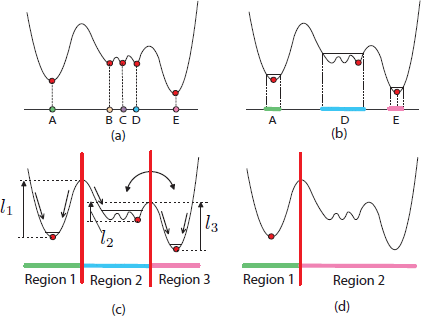
\includegraphics[width=0.5\linewidth]{../resources/watershed/1570179_WS_steps.png}
\caption{
Graphical depiction of Atkar et al.'s Watershed segmentation implementation.\cite{HierSurfSeg_for_autobody_painting}
}
	\label{fig:ws_1570179_steps}
\end{figure}

In figure \ref{fig:ws_1570179_steps} subfigure (a) shows Mangan and Whitaker's step 2: locating and labeling each local minima.
Region 1 in subfigure (c) depicts the original step 5: descent to a minimum, and regions 2 and 3 in the same subfigure show step 6: the merging of shallow regions into deep ones.
The step shown in subfigure (b) is of Atkar et al.'s own design, and due to its adaptation in this work, is described in the section on \textit{minima expansion}.
Figure \ref{fig:ws_1570179_steps} concludes with the end result of Watershed in subfigure (d).

\subsubsection{Region Initialization}
In this work's implementation the curvature values and derivative thereof are calculated once for the whole mesh prior to the first Watershed pass.
Watershed step 0, applying the height function to the mesh, is shown in figure \ref{sfig:ws_dk}.
This work's version of Watershed begins by creating mesh regions from each local minima.
Here, local minima includes local plateaus.
Thus, if a region of the mesh is found whose vertices' curvature are all roughly equal and less than that of their neighbors, it is a minima plateau.

\begin{figure}[htb]
	\centering
	\begin{subfigure}{0.45\textwidth}
		\centering
		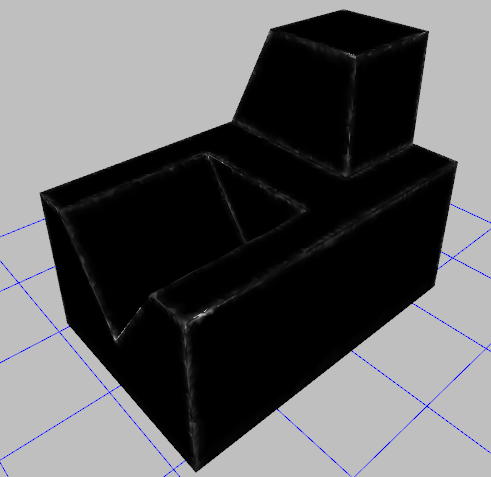
\includegraphics[width=\linewidth]{../resources/watershed/fc028_WS0.png}
		\caption{Watershed step 0: Apply height function to mesh. White indicates high curvature and black indicates low curvature.}
		\label{sfig:ws_dk}
	\end{subfigure}
	\hfill
	\begin{subfigure}{0.45\textwidth}
		\centering
		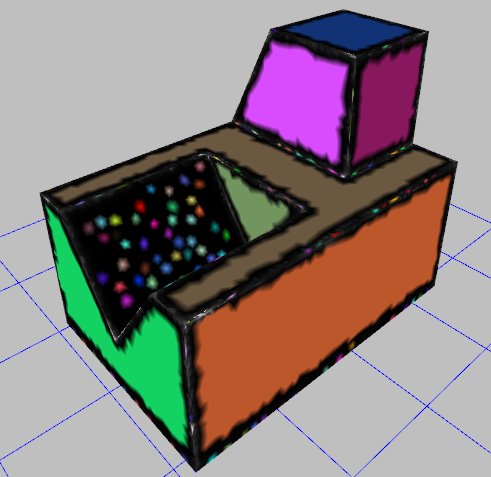
\includegraphics[width=\linewidth]{../resources/watershed/fc028_WS1.png}
		\caption{Watershed step 1: Mesh region initialization. Each color is a separate mesh region.}
		\label{sfig:ws_1}
	\end{subfigure}
\caption{
Watershed segmentation steps 0 and 1 shown applied to test object ``fc028\_e''.
}
\end{figure}

Figure \ref{sfig:ws_1} shows the result of region initialization on the test object ``fc028\_e''.
Because the surfaces of the test object are perfectly flat, the horizontal and vertical surfaces exhibit large plateaus.
The lack of plateaus on the inclined surface is most likely due to floating point errors in the vertex positions on the inclined surface.

\subsubsection{Minima Expansion}
This step was adopted from Atkar et al.'s implementation of Watershed segmentation\cite{HierSurfSeg_for_autobody_painting}.
Each mesh region expands up to a pre-set depth, absorbing any regions encountered.
Although not essential to the segmentation results, it facilitates subsequent steps by effectively filtering high frequency noise and features from the mesh.
It is worth noting that Watershed segmentation overall would work without \textit{minima expansion}, but would be slightly slower because the region merging in steps 4.1 and 4.2 are a little more computationally expensive than region merges during \textit{minima expansion}.

\begin{figure}[htb]
	\centering
	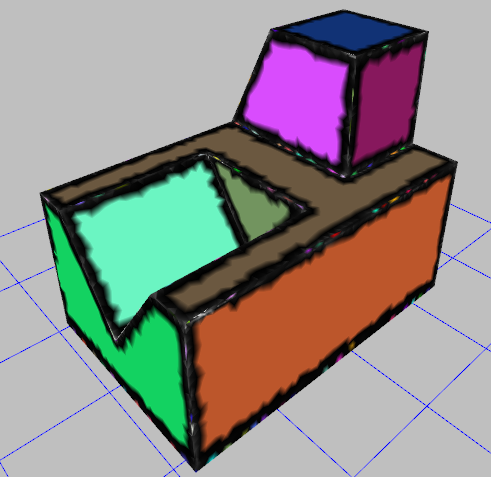
\includegraphics[width=0.5\linewidth]{../resources/watershed/fc028_WS2.png}
\caption{
Test object ``fc028\_e'' post Watershed segmentation step 2.
}
	\label{fig:ws_2}
\end{figure}

Figure \ref{fig:ws_2} shows the result of \textit{minima expansion} on the test object.
Because the variation in height among the vertices of the inclined surface was minimal, one of the initial local minima was able to expand to most of the inclined surface's area.

\subsubsection{Descent to Minima}
From each un-assigned vertex a trail following the path of steepest descent is started.
When a mesh region is encountered, the traversal ends and all path vertices are added to the encountered mesh region.
Plateaus encountered during the descent are added to the traversal path.
In this way, Mangan and Whitaker's step \ref{plateau_step} is effectively split between Region Initialization and Descent to Minima.
A way to visualize this step is by placing an imaginary drop of water at an un-assigned vertex of the object.
All vertices touched by the water droplet as it descends the height map of the object's surface are added to the region that eventually catches the droplet.
Post \textit{descent to minima} all vertices have been assigned to a mesh region and the mesh has been segmented.
Figure \ref{fig:ws_3} shows the result of \textit{descent to minima} on the test object.

\begin{figure}[htb]
	\centering
	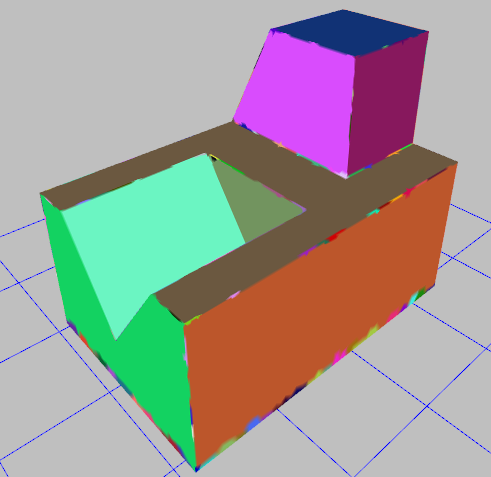
\includegraphics[width=0.5\linewidth]{../resources/watershed/fc028_WS3.png}
\caption{
Test object ``fc028\_e'' post Watershed segmentation step 3: Descent to minima
}
	\label{fig:ws_3}
\end{figure}

\subsubsection{Mini-Merge}
As noted by Mangan and Whitaker, Descent to Minima will segment the given mesh, but in all likelihood it will be overly segmented.
Their solution was to merge shallow regions into adjacent deeper regions (see subsequent section on \textit{shallow merge}).
Through testing small high curvature regions were observed, that due to their high curvature did were not merged into any of the larger more useful regions.
To combat this, the ``Mini-Merge'' step was developed to merge regions deemed too small to be worth keeping.
The merge condition changed throughout development, from a fixed number of vertices threshold, to a threshold relative to the total number of vertices in the mesh undergoing Watershed segmentation, to the condition that the number of perimeter vertices in the region be fewer than 50\% of the region's vertices.
(reword previous sentence?)
The \textit{mini-merge} procedure is shown in algorithm \ref{alg:WS:mini_merge}.

\begin{algorithm}[htb]
\caption{Mini-Merge}\label{alg:WS:mini_merge}
\begin{algorithmic}[1]
\Function{miniMerge}{Mesh sections $S$}
	% \State Sort $S$ by vertex count in ascending order
	\For{$s$ in $S$}
		% \State $s_{small} \leftarrow S$.first
		\If{$s$.small()}
			\State $s_{lowside} \leftarrow s$.findLowSideNeighbor()
			\State $s_{lowside}$.absorb($s$)
			% \State $S$.erase($s$)
		\EndIf
	\EndFor
\EndFunction
\end{algorithmic}
\end{algorithm}

\textit{Mini-merge} iterates through each mesh section, checking each if it meets the aforementioned merge condition.
When a small region is found, the region adjacent its low side is sought, which then absorbs the small region.
% Mesh regions that trigger the merge condition are merged into the mesh region adjacent their shallow side.
The method to find the low-side adjacent neighboring mesh region is shown below in algorithm \ref{alg:MR:low_side_neighbor}.

\begin{algorithm}[htb]
\caption{Find low side neighbor}\label{alg:MR:low_side_neighbor}
\begin{algorithmic}[1]
\Function{findLowSideNeighbor}{}
	\For{$p_{perimeter}$ in $P_{perimeter}$}
		\For{point $p_{adj}$ adjacent to $p_{perimeter}$}
			\If{$p_{adj}$ not in this region AND $p_{adj}$ is in bounds}
				\State \textbf{return} $p_{adj}$.meshRegion
			\EndIf
		\EndFor
	\EndFor
\EndFunction
\end{algorithmic}
\end{algorithm}

The receiving mesh region is found by searching the vertices adjacent to the mini region's lowest perimeter vertex.
If for some reason no valid mesh region adjacent to that vertex is found, the neighborhoods of the remaining perimter vertices are checked in ascending order until a valid mesh region is found.

\begin{figure}[htb]
	\centering
	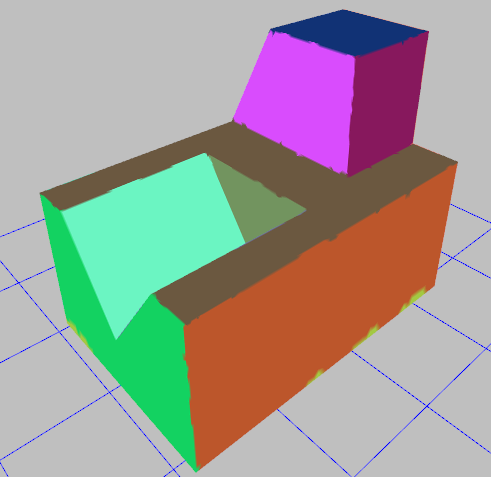
\includegraphics[width=0.5\linewidth]{../resources/watershed/fc028_WS4.1.png}
\caption{
Watershed segmentation step 4.1 shown applied to test object ``fc028\_e''.
}
	\label{fig:ws_4.1}
\end{figure}

As can be seen in figure \ref{fig:ws_4.1} the segmentation results post \textit{mini-merge} are noticeably cleaner than after the previous step.
Had the test object been more complex, the need for further merging would have been apparent.

\subsubsection{Shallow Merge}
This step was adopted without modification from Mangan and Whitaker.
The implementation of \textit{shallow merge} used in this work is detailed in algorithm \ref{alg:WS:shallow_merge}.

\begin{algorithm}[!b]
\caption{Shallow-Merge}\label{alg:WS:shallow_merge}
\begin{algorithmic}[1]
	\Function{shallowMerge}{Mesh sections $S$, real $t_e$}
		\State Sort $S$ by mesh section depth in ascending order
		% \State $d_{th} \leftarrow d_{deepest}^{t_e}$\Comment{See equation \ref{eq:merge_threshold} for explanation}
		\State calculate merge threshold $d_{th}$
		\While{$S$.first.depth < $d_{th}$}
			% \State \Comment{While the depth of the shallowest mesh is below the merge threshold}
			\State $s_{shallow} \leftarrow S$.first
			\State $s_{lowside} \leftarrow s_{shallow}$.findLowSideNeighbor()
			\State $s_{lowside}$.absorb($s_{shallow}$)
			% \State $M$.erase($m_{shallow}$)
			\State $s_{lowside}$.updateDepth()
		\EndWhile
	\EndFunction
\end{algorithmic}
\end{algorithm}

First the mesh sections are sorted by depth in ascending order, so that as soon as the first mesh section is above the merge threshold, the others are guaranteed to be above it as well.
On line 3 \verb|ShallowMerge|'s second argument $e$ is used in equation \ref{eq:merge_threshold} to calculate the merge threshold $d_{th}$.
\begin{equation}\label{eq:merge_threshold}
	d_{th} = d_{max}^{e}
\end{equation}
where $d_{max}$ is the depth of the deepest region and $e$ is the threshold value provided to \textit{shallow-merge}.
Due to the threshold value being applied as an exponent, values greater than 1 are pointless.
Regions with a depth below the merge threshold are merged into the mesh region adjacent their shallow side, using the algorithm \ref{alg:MR:low_side_neighbor}.
The \textit{mini-merge} and \textit{shallow-merge} procedures are quite similar, with the main difference being that the absorbing mesh section in \textit{shallow-merge} must update its depth in order to maintain the depth ordering.

\begin{figure}[htb]
	\centering
	\begin{subfigure}{0.45\textwidth}
		\centering
		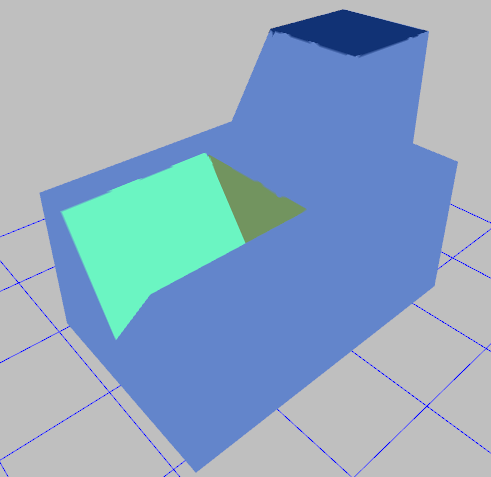
\includegraphics[width=\linewidth]{../resources/watershed/fc028_WS4.2.0.png}
		\caption{Shallow merge with a high merge threshold}
		\label{sfig:ws_4.2.0}
	\end{subfigure}
	\hfill
	\begin{subfigure}{0.45\textwidth}
		\centering
		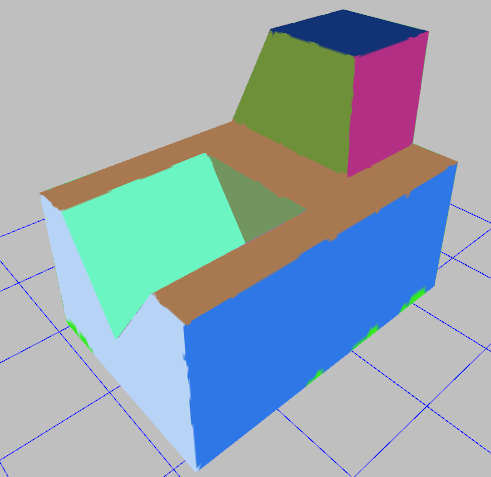
\includegraphics[width=\linewidth]{../resources/watershed/fc028_WS4.2.1.png}
		\caption{\raggedright Shallow merge with a lower merge threshold}
		\label{sfig:ws_4.2.1}
	\end{subfigure}
\caption{
Results from Watershed segmentation step 4.2 with a high merge threshold (a) and a lower merge threshold (b).
}
\end{figure}

Figures \ref{sfig:ws_4.2.0} and \ref{sfig:ws_4.2.1} show the results post \textit{shallow-merge}.
If the merge threshold is too high, useful regions will be merged together into a large composite mesh section, as can be seen in figure \ref{sfig:ws_4.2.0}.
figure \ref{sfig:ws_4.2.1} shows the result of a merge threshold more appropriate for the mesh shown.
Because each model has different geometry and meshing, a certain merge threshold may work well for one model, yet work poorly for another.
A certain merge threshold may not even work well for the entirety of a single model.
This is why the \textit{3D Segmentation} process is iterative.
By starting with a relatively high merge threshold exponent (0.95) and decreasing, all surfaces should eventually be classified as a certain primitive.

\subsubsection{Boundary Smoothing}
This step is more post-processing and ``cleaning'' of the mesh region boundary than actual segmentation.
Due to randomness in the mesh there are situations where a vertex is connected to its region by a single edge.
Such vertices are named ``web1'' points, due to them having a single webbed connection to their region's perimeter.
In order to smooth the region boundary, an attempt is made to find an adjacent mesh region more suitable to possess each web1 point.
Because vertices with only 3 edges are exceedingly rare in well meshed models, it is sufficient to transfer ownership of the web1 point to the adjacent region with the highest number of connecing edges.
Thus, for example, A vertex assigned to region 4 through Minima Descent with edges connecting to regions 4, 10, 12, and 12, would be transferred to region 12.
No explicit tie breaking mechanism was deemed necessary, but lower numbered regions are likely given priority due to how the code was written.
% At one point perimeter vertices with 3 or more connections to other same-region perimeter vertices were considered a problem,...

% TODO: take a pair of screenshots to illustrate WS5:boundary smoothing?

\subsection{Surface Classification}
Mesh regions received from Watershed segmentation need to be classified so that the appropriate UV-map is assigned to them.
The primitives against which each mesh region is tested are: planes, cylinders, and ellipsoids.
Because Watershed segments along regions of high curvature, perimeter vertices were excluded from the tests described below.
The main idea was to perform some tests on a the mesh region's vertices to obtain an educated guess as to the surface's class, and confirm or reject the guess by attempting to fit the assumed shape to the surface and examining the resultant error value.
This works well for planar classification because measuring the distance of a given point from the regression plane is trivial.
Computing the distance from a given point to an ellipse or other conic shape is non-trivial and, at the time of writing, no exact algebraic solution was found.
In place of an exact distance function, the sum of squared residuals was used.
For example, a point on a conic section should satisfy equation \ref{eq:gen_conic}, but for a point \textit{almost} on a conic section, the result will be non-zero:
\begin{equation}
	R(x,y) = Ax^2 + Bxy + Cy^2 + Dx + Ey + F,
\end{equation}
where $R(x,y)$ is the residual. The error function then becomes:
\begin{equation}
	e = \sum_i \left(Ax_i^2 + Bx_i y_i + Cy_i^2 + Dx_i + Ey_i + F\right)^2
\end{equation}
While easy to calculate, this value is unreliable as an indicator of whether or not the given surface is actually a conic surface.
Through testing cases were in which obviously non-cylindric surfaces yielded extremely low error values.
Due to this realization greater emphasis was placed on the initial classification step.

\subsubsection{Planar Classification}
Various tests were devised to determine if a given mesh region can be classified as planar.
An early idea was to cluster the normals of the given mesh region, and perform a sort of statistical analysis on them.
By clustering all normals within a set allowable deviation, the spread in the number of vertices in each cluster should provide insight into the surface type.
One would expect a plane to have a normal-cluster with an overwehelming number of vertices relative to other normal-clusters produced.
By comparison, a cylinder would be expected to have multiple ``significant'' normal-clusters, with similar vertex counts.
This idea was later deemed unnecessarily complex and too susceptible to mesh deviations, and retired in favor of other ideas.

Another idea was to calculate an overall normal vector by performing Principal Component Analysis (PCA) on the vertices' normals.
The vertice's normals were then compared to this overall normal via their dot product.
If too many vertex normals deviated beyond a set angular threshold, the mesh region was determined to be non-planar.
This test works well for ``perfect'' models, such as those from CAD, but is less useful when dealing with noisy meshes and can yield false negatives.

Later, a test that compared the vertices' mean principal curvatures against set thresholds was developed.
Theoretically, the vertices in a planar mesh would exhibit 0 curvature.
Thus, the vertices' 1st principal curvature could be compared against a near-zero threshold, with those above the threshold rejected as non-planar.
Again, this works well for ``clean'' geometry, but not for noisy meshes, because even small deviations in the mesh can inflate the mean curvature.
It \textit{is} possible to set useful curvature thresholds for noisy meshes, but they will be significantly higher than those set for clean meshes, meaning the test does not generalize between clean and unclean meshes.

The second planar test was deemed the most reliable and is used in the submitted algorithm.
As a check on the test, planar regression via Singular Value Decomposition is performed on the mesh region's vertices, and the root mean squared error is reported.
If the RMSE is within a set threshold, the region passes the second check and is classified as planar.

NOTE: perhaps talk about other (untested) ideas?

\subsubsection{Cylindric Classification}
``Cylinder'' (and cylindric) in this context means a surface whose cross section is a conic shape, and has a single axis.
% The single axis criterion was central to later tests conceived during development.

As mentioned in the planar classification section, an early idea was to perform statistical analysis on clustered normals.
An issue with using that method for cylindric classification is that a sphere and a cylinder would yield similar normal-cluster histograms.
(I could probably go into greater detail about why this was a foolish notion, but i would rather write about ideas that had a higher chance of success.)

A test that examined the mean principal curvature values of the mesh region was also considered, but it failed to prove useful for the same reasons outlined in Planar Classification(ref?).
Theoretically, the first principal curvature on the surface of a cylinder would fulfill $|\kappa_1| >> 0$ and the second principal curvature would be approximately 0.
Setting reliable thresholds proved overly difficult.

Another test sought to make use of the vertices' normals by determining the axis direction via PCA, and checking that the dot product between each vertex's normal and the axis was roughly 0:
\begin{equation}
	\vec{v}_{axis} \cdot \vec{n_i} \approx 0.
\end{equation}
This approach has 2 glaring flaws: planes pass this test, and cones do not pass.
% Various tests that take into account the vertices' normals were conceived, but all were either abandoned due to inefficacy, or simply unimplemented due to time constraints.

Currently, the test chosen for planar classification doubles as a cylindric identification.
If a mesh region fails that test, it is non-planar, and thus most likely cylindric.

(?) Talk about future ideas?

? talk about other flaws? This was definitely a weak point in my work

\subsubsection{Ellipsoidal Classification}
The third primitive type would have been ellipsoids, but due to their complexity and time constraints no ellipsoidal indentification or classification functions were developed.
Theoretically, the prinicipal curvature values could also be applied here.
An ellipsoid curves in both surface directions, thus both $|\kappa_1|$ and $|\kappa_2|$ should be noticeably greater than 0.

A flaw with the cylindric tests and this principal curvature test is that they are unable to differentiate between the target surface class and a composite shape.

\section{Geometry Simplification}

\begin{figure}[htb]
	\centering
\begin{tikzpicture}[inner sep=0,
	vertex/.style={circle, radius=2pt,fill, inner sep=2pt,outer sep=0pt}]
	% Nodes
	\matrix (table) [
		matrix of nodes,
		nodes in empty cells,
		row sep=8mm, column sep=6mm,
		nodes={anchor=center}
	] {
		\node[text width=24mm] (MRs) {Classified Mesh Sections}; &[7mm]
		\node[FC-Node, text width=20mm, minimum size=15mm] (cEdges) {Create shared edges}; &
		\node[FC-Node, text width=20mm, minimum size=15mm] (exEdges) {Extend shared edges}; &
		\node[FC-Node, text width=20mm, minimum size=15mm] (cSurfaces) {Create simple surfaces}; &
		\node[text width=24mm, align=left] (SSurfaces) {Simplified Surfaces}; \\
		& & & & \\
	};
\node[FC-Node, fit=(table-2-2)(table-2-3),minimum size=7mm, text width=46mm,label={center:Create shared corners}] (cCorners) {};
	% Connections
	\draw[FC-Arrow] (MRs) -- (cEdges)
		node[pos=0.7, vertex] (split) {};
	\draw[FC-Arrow] (split) -- ($(split |- cEdges.north west)+(0,0.3)$) -| (cSurfaces.north)
		node[pos=0.5] (top) {};
	\draw[FC-Arrow] (cEdges.south) -- (cEdges.south |- cCorners.north);
	\draw[FC-Arrow] (cEdges) -- (exEdges);
	\draw[FC-Arrow] (cEdges) -- (exEdges);
	% \draw [FC-Arrow] ($(cEdges.east)+(0,0.4)$) -- ($(cSurfaces.west)+(0,0.4)$);
	\draw[FC-Arrow] (cCorners.north -| exEdges.south) -- (exEdges.south);
	\draw[FC-Arrow] (exEdges) -- (cSurfaces);
	\draw[FC-Arrow] (cSurfaces) -- (SSurfaces);
	% GeoSimp container node
	\node[thick, dashed,draw, rounded corners=8pt,inner sep=7pt, fit=(split)(top)(cCorners)(cSurfaces),label={90:Geometry Simplification}]{};
\end{tikzpicture}
	\caption{Graphic depiction of the 3D segmentation procedure. Simple surfaces require both shared edges and shared corners, hence the connection from each.}
	\label{fig:GeoSimp}
\end{figure}

The purpose of the geometry simplification step is to create a simplified form for each mesh region provided by Segmentation 3D.
Geometry Simplification's output is a set of ``simple surfaces'' created from the provided mesh regions.
A simple surface contains, among other things, a reference to the mesh region from which it was created, a UV-map, and the unwrapped 2D region outline.
Geometry Simplification follows the block diagram shown in figure \ref{fig:GeoSimp}.
First the \verb|SharedEdges|, edges between mesh regions, are ascertained.
These are used to determine the region corners (``shared corners''), which are then used to finish preparing the shared edges (Extend shared edges).
Finally, the completed shared edges plus the mesh regions are used to create the \verb|simple surfaces|, which are passed on to the next high-level step.

\subsection{Create Shared Edges}
The boundary between two mesh regions is termed a ``shared edge'', because its information is shared between the two mesh regions it divides.
Each shared edge is made up of a list of line segments that approximate the boundary between two mesh regions.
The algorithm to obtain the shared edges is shown split into algorithms \ref{alg:shared_edges_1} and \ref{alg:shared_edges_2}.
The function \textbf{CreateSharedEdges()} can be broken into \textbf{edge discovery} and \textbf{edge refinement}.
% Line 2 sets up list $E_{points}$, in which each entry $i$ is the list of all points for the $i-th$ discovered edge.
% $E_{points}$ is filled throughout \textbf{edge discovery} and in \textbf{edge refinement}
In \textbf{edge discovery} the list of vertices found along each edge is appended to list $E_{points}$.
In \textbf{edge refinement} each edge's list of vertices in $E_{points}$ is transformed into a concise shared edge.

\begin{algorithm}[!htb]
	\caption{createSharedEdges() Part 1: Edge discovery}\label{alg:shared_edges_1}
\begin{algorithmic}[1]
\Function{createSharedEdges}{Surfaces $S$, UV-maps $M$}
	\State new list $E_{points}$ \Comment{Each entry is an edge's list of points}
	% "edge discovery" section
	\State new set $P_{remaining} \leftarrow$ all mesh region perimeter points
	\While{$P_{remaining}$ not empty}\label{alg:shared_edges:while_k_remaining}
		\State point $p_{edge} \leftarrow$ first value in $P_{remaining}$
		\State new queue $K_{tips} \leftarrow p_{edge}$ \Comment{For the beginning of each edge}
		\While{$K_{tips}$ not empty}\label{alg:shared_edges:while_k_tips}
			\State $e_{start} \leftarrow K_{tips}$.dequeue()
			\State \textbf{skip if} $e_{start}$ already in $E_{points}$
			\State new list $P_{edge}$ \Comment{List of points in the current edge}
			\State new queue $P_{search}$ \Comment{Queue of points to search along current edge}
			\While{$P_{search}$ not empty}
				\State $p_{edge} \leftarrow P_{search}$.dequeue()
				\State \textbf{skip if} $p_{edge}$ already in $P_{edge}$
				\State $P_{edge}$.append($p_{edge}$)
				\For{$p_{adj}$ in $p_{edge}$.adjacent\_points}
					\If{$p_{adj}$ on current region boundary}
						\State $P_{search}$.enqueue($p_{adj}$)
					\EndIf
					\If{$p_{adj}$ adjacent to 3+ regions}
						\State $K_{tips}$.enqueue(EdgeStart from $p_{adj}$)
					\EndIf
				\EndFor
			\EndWhile
			\State Remove $P_{edge}$ points from $P_{remaining}$
			\State $E_{points}$.append($P_{edge}$)
		\EndWhile
	\EndWhile
	\algstore{create_shared_edges}
\end{algorithmic}
\end{algorithm}

The \textbf{edge discovery} section, spanning lines 3-28, consists of traversing each mesh section boundary to collect all vertices relevant to that edge and storing them in a list in $E_{points}$.
The outermost \verb|while| loop, beginning on line \ref{alg:shared_edges:while_k_remaining}, ensures that all perimeter points, of all mesh regions, are accounted for.
Each cycle of this loop completely processes a single edge graph.
Edge graph in this context means the collection of edges that are linked to one another.
For example, a cube has a single edge graph, whereas a cylinder has 2 edge graphs, each containing a single edge.
The queue $K_{tips}$ stores potential edge starts.
The next \verb|while| loop, on line \ref{alg:shared_edges:while_k_tips}, processes each potential edge start in $K_{tips}$.
Because multiple edge starts could describe the same edge, it is necessary to check if the current edge start $e_{start}$ is already contained in an edge in $E_{points}$ (line 9).
The queue $P_{search}$ created on line 11 handles the points found to be on the current edge.
The subsequent \verb|while| loop processes $P_{search}$ until empty, first checking for duplicates, appending the current edge point $p_{edge}$ to the list of current edge points $P_{edge}$, and finally checking its neighbors for new edge points.
A vertex is deemed to be on the edge between regions $A$ and $B$ if it is either in $A$ and adjacent to $B$ or in $B$ and adjacent to $A$.
Lines 20-22 show that if a vertex adjacent to 3 or more regions is found, an edge start is created from it and enqueued to $K_{tips}$.
After $P_{search}$ is exhausted, $P_{edge}$ is assumed to contain all points on the current edge.
These points are then removed from the overall point set $P_{remaining}$ and appended to $E_{points}$, concluding the $K_{tips}$ \verb|while| loop.

\begin{algorithm}[htb]
	\caption{CreateSharedEdges() Part 2: Edge refinement}\label{alg:shared_edges_2}
\begin{algorithmic}[1]
	\algrestore{create_shared_edges}
	% "edge refinement" section
	% \State comment about source of muv1/2
	\State new list $E$ \Comment{List of shared edges}
	\For{$P_{edge}$ in $E_{points}$}\label{alg:edge_refinement_for}
		\State Determine the surfaces $s_1$ and $s_2$ adjacent current point line $P_{edge}$
		\State Obtain UV-maps $m_{UV1}$ and $m_{UV1}$ from $s_1$, $s_2$ and $M$
		\State ClampPointsToSurfaces($P_{edge}$, $m_{UV1}$, $m_{UV2}$)\label{alg:edge_refinement_clamp_pts}
		\State SortEdgePoints($P_{edge}$)
		\State $E$.append(SharedEdge($P_{edge}$))
	\EndFor
	\State \textbf{return} $E$
\EndFunction
\end{algorithmic}
\end{algorithm}

\textbf{Edge refinement} is, relative to \textbf{edge discovery}, fairly simple.
A new list $E$ is created to store the final shared edges.
The \verb|for| loop on line \ref{alg:edge_refinement_for} iterates through the lists of edge vertices in $E_{points}$, attempting to create a shared edge from each.
On line \ref{alg:edge_refinement_clamp_pts} \verb|ClampPointsToSurfaces()| forces the edge points onto an idealized representation of the two bordering mesh sections.
For an edge between two planar surfaces, this would force all points to be colinear.
Next the clamped points are sorted according to position along the line using \verb|SortEdgePoints()|.
Finally a shared edge is created from the edge points, and then appended to $E$.
Within the creation of a shared edge the RDP algorithm is used to simplify the line down to only the critical points.
% The complete list of vertices is simplified via the Ramer-Douglas-Peucker (RDP) algorithm\cite{RDP_line_reduction}.
The mesh's mean edge length is used as the tolerance width in the RDP algorithm.
Once all point lists in $E_{points}$ have been processed, the list $E$ is returned, and \verb|CreateSharedEdges()| is complete.

\subsection{Create Shared Corners}

\begin{algorithm}[!b]
	\caption{Create shared corners}\label{alg:shared_corners}
\begin{algorithmic}[1]
\Function{createSharedCorners}{Region edges list $E_{R,E}$}
	\State new list $C$ \Comment{To store the shared corners}
	\For{$E_r$ in $E_{R,E}$}
		\State new list $T$ \Comment{Set of all line tips relevant to a given region}
		\For{edge $e$ in $E_r$}
			\State $T$.append($e$.start)
			\State $T$.append($e$.end)
		\EndFor
		\While{$T$ not empty}
			\State new line tip $t_{target} \leftarrow$ first in $T$
			\State $T$.erase($t_{target}$)
			\State new line tip $t_{near} \leftarrow T$.closestTo($t_{target}$)
			% \State new line tip $t_{near} \leftarrow$ first in $T$
			% \State new point $p_{target} \leftarrow l_{target}$.position
			% \State new float $d \leftarrow \infty$
			% \For{$t$ in $T$} \Comment{Find the line tip closest to $t_{target}$}
			% 	\State new point $p \leftarrow t$.position
			% 	\If{distance($p_{target}$, $p$) < $d$}
			% 		\State $d \leftarrow$ distance($p_{target}$, $p$)
			% 		\State $t_{near} \leftarrow t$
			% 	\EndIf
			% \EndFor
			% check existing shared corners if any contain near/target l
			\State new boolean $b_{found} \leftarrow$ false
			\For{$c$ in $C$}
				\If{$c$.contains($t_{target}$) or $c$.contains($t_{near}$)}
					\State $c$.insert($t_{target}$)
					\State $c$.insert($t_{near}$)
					\State $b_{found} \leftarrow$ true
					\State \textbf{break}
				\EndIf
			\EndFor
			\If{not $b_{found}$}
				\State new shared corner $c$($t_{target}$, $t_{near}$)
				\State $C$.append($c$)
			\EndIf
			\State $T$.erase($t_{near}$)
		\EndWhile
	\EndFor
	\State \textbf{return} $C$
\EndFunction
\end{algorithmic}
\end{algorithm}

Shared corners are used to simplify the process of extending the shared edges to the regions they abut.
The process of creating shared corners $C$ is outlined in algorithm \ref{alg:shared_corners}.
The \verb|CreateSharedCorners()| argument $E_{R,E}$ is a list, where each entry is the list of edges that border the mesh region indexed by the $E_{R,E}$ index.
That is, the $i$-th item in $E_{R,E}$ is the list of edges that border mesh region $i$.
Determining which line tips match is facilitated by each item in $E_{R,E}$ only containing the edges relevant to a given mesh region.
% Having a list of the edges relevant to a single mesh region facilitates determining which line tips match.

% \verb|CreateSharedCorners()| is primarily a \verb|for| loop loop
Each iteration of the main \verb|for| loop attempts to create corners from that region's edges.
% The \verb|for| loop starting on line 3 iterates through each list of edges $E_r$ in $E_{R,E}$.
Lines 4-8 create the set $T$ of line tips and initialize it with both line tips from each edge in $E_r$.
The \verb|while| loop starts by finding a pair of matching line tips (lines 10-12).
% Lines 10-12 pull the first line tip from $T$ and find the closest line tip to the removed one.
% The remainder of the while loop serves to check if any existing shared corner $c$ in $C$ already contain either of the matching line tips $t_{target}$ or $t_{near}$.
Next an existing shared corner $c$ that already contains either matching line tip is sought.
If such a shared corner is found $t_{target}$ and $t_{near}$ are added to it.
Otherwise a new shared corner is created from the matching line tips and appended to $C$.
Finally, the list of shared corners $C$ is returned.

\subsection{Extend Shared Edges}
% Another meaningful name for this would be "force line tip coincidence", at least for the fn
At this point the shared edges align with the regions they divide, but likely do not extend to meet the shared corners or each other.
\verb|ClampLineTips()|, described in algorithm \ref{alg:clamp_line_tips}, exists to rectify this.

\begin{algorithm}[hb]
\caption{Clamp Line Tips}\label{alg:clamp_line_tips}
\begin{algorithmic}[1]
\Function{clampLineTips}{$C$, $S$, $M_{UV}$}
	\For{$c$ in $C$}
		\State new set $S_{corner} \leftarrow c$.adjoiningSurfaces() \Comment{The set of surfaces that adjoin $c$}
		\For{line tip $t$ in $c$.lineTips()}
			\State new set $S_{edge} \leftarrow E$[$t$].adjacentRegions()
			\State new set $S_{diff} \leftarrow S_{corner} - S_{edge}$ \Comment{The set difference of $S_{corner}$ and $S_{edge}$}
			% \State new uint $i_{UV} \leftarrow S$[$S_{diff}$.first].UVMapIndex
			\State Obtain new UV-map $m_{UV}$ representing $S_{diff}$ from $M_{UV}$
			% \State new UV-map $m_{UV} \leftarrow M_{UV}$[$i_{UV}$]
			% \State $E$[$t$.edgeIndex].clampTipPoint($m_{UV}$, $t$.tipType)\label{alg:clamp_tip_point}
			\State $t$.clampTipPoint($m_{UV}$)\label{alg:clamp_tip_point}
		\EndFor
	\EndFor
\EndFunction
\end{algorithmic}
\end{algorithm}

The \verb|ClampLineTips| arguments are as follows:
% $E$: the shared edges,
$C$: the shared corners, $S$: the mesh surfaces, and $M_{UV}$: the list of UV-maps.
% The objective is to find for a given line tip the region, and its corresponding UV-map, that set the line tip's position along the line tip direction.
The objective is to find the surface that a given line tip points to, and use that surface's UV-map to force the line tip onto said surface.
The inner \verb|for| loop iterates through the line tips of the current shared corner.
To determine to which surface a line tip points, the set $S_{edge}$ of surfaces adjacent to the line tip $t$ is subtracted from the set $S_{corner}$ of surfaces adjacent to the current shared corner $c$.
% For a typical 3-surface corner, the set difference $S_{diff}$ will contain a single element,
The number of elements in the set difference $S_{diff}$ is dependent on the number surfaces joined by the current shared corner.
Although $S_{diff}$ can contain more than one element, it matters not which is chosen as the extension target for the line tip.
Next the UV-map belonging to the surface in $S_{diff}$ is obtained.
On line \ref{alg:clamp_tip_point} the line tip $t$ is forced to lie at the intersection of its tangent and the extension target surface.
Figure \ref{fig:extend_shared_edges} below shows the before and after of applying \verb|ClampLineTips| to a set of shared edges.

\begin{figure}[htb]
	\centering
	\begin{subfigure}{0.45\textwidth}
		\centering
		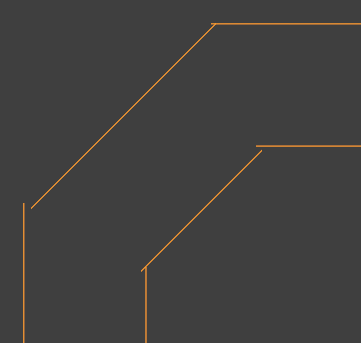
\includegraphics[width=\linewidth]{../resources/geo_simp/1505020_shared_edges.png}
		\caption{Shared edges post \textit{create shared edges}}
		\label{sfig:gs_shared_edges}
	\end{subfigure}
	\hfill
	\begin{subfigure}{0.45\textwidth}
		\centering
		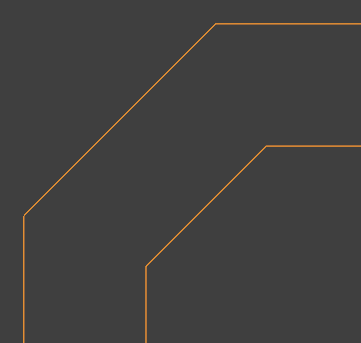
\includegraphics[width=\linewidth]{../resources/geo_simp/1505020_shared_edges_clamped.png}
		\caption{Shared edges post \textit{extend shared edges}}
		\label{sfig:gs_shared_edges_clamped}
	\end{subfigure}
\caption{
The shared edges from test object ``1505020'' Before and after \textit{extend shared edges}
}
	\label{fig:extend_shared_edges}
\end{figure}

As can be seen in figure \ref{sfig:gs_shared_edges} ``unclamped'' shared edges are decent, but noticeably unconnected.
Figure \ref{sfig:gs_shared_edges_clamped} shows the same edges post \textit{extend shared edges} and noticeably connected.

\subsection{Create Simple Surfaces}
A simple surface is created from a mesh region and the shared edges that border said mesh region.
% How are simple surfaces formed?
The bulk of the procedure to create a simple surface is the process to form the surface's outlines from the given shared edges.
This process is described in detail in algorithm \ref{alg:find_outlines}.
% Given a mesh region and the previously created shared edges as input, the simple surface first collects the edges and corners that border the source mesh region.
% Next the outlines of the mesh region are generated from the shared edges (see below...)

% find_outlines(shared_corners, corner_indices, edge_indices, uv_map_index, uv_mappings);
\begin{algorithm}[!htb]
	\caption{Find outlines}\label{alg:find_outlines}
\begin{algorithmic}[1]
\Function{findOutlines}{Shared edges $E_{shared}$, Line tips $T$, UV-map $m$}
	\State new set O \Comment{To store the created outlines}
	\State new list $T_{sorted} \leftarrow T$ \Comment{Local copy of $T$ to be sorted throughout function}
	% \State new uint $vii \leftarrow 0$
	\State new set $E$ from each edge associated with $T$

	\While{$E$ not empty}
		\State new list $T_{outline}$ \Comment{For the outline's line tips}
		\State new edge $e_0 \leftarrow E$.first
		% \State new line tip $t_{target} \leftarrow$ LineTip{$e_0$, END}
		\State new line tip $t_{target}$ derived from END of $e_0$
		\Repeat
			\State $t_{target} \leftarrow$ findNextLineTip($t_{target}$, $E_{shared}$)
			\State $T_{outline}$.append($t_{target}$)
			\State $E$.erase($t_{target}$.edge)
		\Until{$t_{target}$.edge = $e_0$}
		\State Update $T_{sorted}$ from $T_{outline}$
		\State new list $P_{corner}$
		\For{$t$ in $T_{outline}$}
			\State new list $P$ from $t$'s shared edge's points
			\If{$t$ is a line tip END}
				\State reverse(P)
			\EndIf
			\For{$p$ in $P$}
				\State new $p_{UV} \leftarrow m$.transformToUV($p$)
				\State $P_{corner}$.append($p_{UV}$)
			\EndFor
		\EndFor
		\State $O$.append($P_{corner}$)
	\EndWhile
	\State $T \leftarrow T_{sorted}$
	\State \textbf{return} $O$
\EndFunction
\end{algorithmic}
\end{algorithm}

The purpose of \verb|FindOutlines| is to determine all outlines associated with the simple surface under construction.
An outline in this context is the surface's boundary lines \textit{and} any holes the surface may have.
Line 4 sets up the set of edges associated with line tips $T$.
Each iteration of the function's \verb|while| loop produces a new outline.
On line 8 a line tip $t_{target}$ is created as the end line tip of edge $e_0$.
This serves as the initial line tip ``targeted'', and as the end condition for the \verb|repeat-until| loop.
The function to find the next sequential line tip, \verb|findNextLineTip|, is shown in algorithm \ref{alg:next_line_tip}.
When a new $t_{target}$ is found it is added to the outline and its edge is erased from $E$ to show that it has been accounted for.
When $t_{target}$'s edge equates to $e_0$ the loop and outline are complete.
The remainder of the \verb|while| loop converts the outline as a list of line tips to a list of points.
On line 17 $P$ is the list of points from the shared edge associated with line tip $t$.
For a straight line this is only 2 points, but for a curve there could be a much larger number of points.
The \verb|if| statement on line 18 ensures that the outline's points are properly sequential, by reversing $P$ if the associated line tip is an END line tip.
Once $P$ is complete, each point $p$ therein	is transformed to the surface's local coordinate system and appended to $P_{corner}$.
The completed list of local points is then added to	the list of outlines $O$.
Once all edges in $E$ have been accounted for in an outline, the outlines are returned and the function finished.
% The outlines created are sorted by descending area size, so that the first outline is guaranteed to be the surface's outline and the remaining outlines are holes in the surface.

\begin{algorithm}[htb]
	\caption{Find next line tip}\label{alg:next_line_tip}
\begin{algorithmic}[1]
\Function{findNextLineTip}{Line tip $t_{target}$, edges $E$}
	\State new point $p_{target} \leftarrow$ position of $t_{target}$
	\State new real $d_{nearest} \leftarrow \infty$
	\State new line tip $t_{nearest}$
	\For{$e$ in $E$}
		\For{$t_{type}$ in [START, END]}
			\State new line tip $t_{temp}$ from $e$ and $t_{type}$
			\State new real $d \leftarrow$ distance from $p_{target}$ to $t_{temp}$'s position
			\If{$t_{temp}$ is not $t_{target}$ AND $d$ < $d_{nearest}$}
				\State $d_{nearest} \leftarrow d$
				\State $t_{closest} \leftarrow t_{temp}$
			\EndIf
		\EndFor
	\EndFor
	\If{line tip $t_{nearest}$ is START type}
		\State \textbf{return} line tip from END of $t_{nearest}$.edge
	\Else
		\State \textbf{return} line tip from START of $t_{nearest}$.edge
	\EndIf
\EndFunction
\end{algorithmic}
\end{algorithm}

The purpose of \verb|findNextLineTip| is to find the next sequential line tip given the current one ($t_{target}$) and a list edges.
% To do so, the line tip closest but not equal to $t_{target}$ is sought,...from the given list of edges.
The nested \verb|for| loops iterate both ends of each edge in $E$ to find the line tip closest but not equal to $t_{target}$.
This yields the sequential next edge, but $t_{nearest}$ is not the line tip sought, because it is still approximately coincident to $t_{target}$.
Thus, the line tip sought, is the one \textit{opposite} along the edge of $t_{nearest}$.
Hence the \verb|if-else| statements on lines 15-18.

Once the creation of simple surfaces is complete, they are passed on to the next high-level step: \textit{2D Segmentation}.
(Is there anything else i should say about simple surfaces?)

\section{2D Segmentation}

\begin{figure}[ht]
	\centering
\begin{tikzpicture}%[inner sep=0]
	\newdimen\dx
	\dx=6mm
	% nodes
	\node[align=center,text width=16mm,inner sep=0] (Outlines) {Simple Surface 2D Shape};
	\node[shape=diamond,aspect=2.0,draw,right=of Outlines] (Convex) {Convex?};
	\node[FC-Node, text width=15mm] (VG) [below=of Convex] {Create Vertex Graph};
	\node[FC-Node, text width=15mm] (ExtIntEdges) [right=\dx of VG] {Extend Interior Edges};
	\node[FC-Node, text width=17mm] (PG) [right=\dx of ExtIntEdges] {Create Polygon Graph};
	\node[FC-Node,text width=30mm] (CMOs) [below=10mm of VG, xshift=7mm] {Generate Convex Merge Options};
	\node[FC-Node,text width=26mm] (OptimalSet) [right=\dx of CMOs] {Determine Optimal Set};
	\node[vertex,right=of PG] (Join) {};
	\node[text width=20mm,right=of Join] (CvPolys) {Convex Polygons};
	% connections
	\draw [FC-Arrow] (Outlines) -- (Convex);
	\draw [FC-Arrow] (Convex) -| (Join) node[pos=0.06,anchor=south] {Yes};
	\draw [FC-Arrow] (Convex) -- (VG) node[pos=0.4,anchor=west] {No};
	\draw [FC-Arrow] (VG) -- (ExtIntEdges);
	\draw [FC-Arrow] (ExtIntEdges) -- (PG);
	\draw [FC-Arrow, rounded corners=5pt] (PG) |-| (CMOs);
	\draw [FC-Arrow] (CMOs) -- (OptimalSet);
	\draw [FC-Arrow] (OptimalSet) -| (Join);
	\draw [FC-Arrow] (Join) -- (CvPolys);
	% Seg2D container node
	\node[thick,dashed,draw,rounded corners=8pt,inner sep=7pt,fit=(Convex)(Join)(CMOs),label={90:2D Segmentation}]{};
\end{tikzpicture}
\caption{Graphic depiction of the 2D segmentation procedure. Non-convex outlines undergo the \textit{interior edge extension} procedure to produce ``optimal'' convex polygons. Convex polygons need not be processed.}
	\label{fig:Seg2D}
\end{figure}

The purpose of \textit{2D Segmentation} is to decompose non-convex polygons into convex polygons whose geometry is more conducive to local path planning.
The \textit{2D Segmentation} step is applied to each simple surface's 2D shape.
During the research phase of the project it was decided that the algorithm to achieve this would be the ``Interior Extension of Edges'' presented by Nielsen et al.\cite{IntEdgeExt}.
Figure \ref{fig:Seg2D} gives a graphical representation of the \textit{2D Segmentation} procedure.

The process can be summarized as the following:
\begin{enumerate}
	\item A vertex graph is created from the input polygon, where each vertex is a node and the polygon's edges are also the graph's edges.
	\item Interior corners are identified, and the interior edges at those vertices are extended, creating new nodes and edges.
	\item The completed vertex graph is then traverse to form a polygon graph, where each node is an atomic convex polygon.
		The 2D edges shared between two polygon nodes double as the graph edges between them.
	\item The set of ``convex merge options'' are generated from the polygon graph.
	\item The subset of convex merge options that minimizes the sum of convex merge option widths is found.
\end{enumerate}
These steps are explained in greater detail in the following subsections.
To illustrate this process, the following test polygons will be used.

\begin{figure}[htb]
	\centering
	\begin{subfigure}{0.48\textwidth}
		\centering
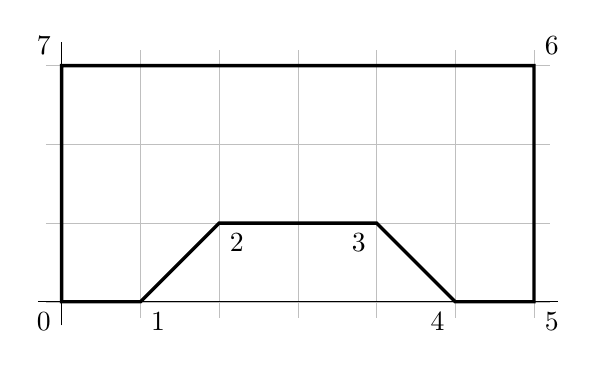
\begin{tikzpicture}
	\draw[step=10mm,gray!50,very thin] (-0.2,-0.2) grid (6.2,3.2);
	\draw (-0.3,0) -- (6.3,0);
	\draw (0,-0.3) -- (0,3.3);
	\draw[very thick] (0,0) node [anchor=north east] {0} --
		(1,0) node [anchor=north west] {1} --
		(2,1) node [anchor=north west] {2} --
		(4,1) node [anchor=north east] {3} --
		(5,0) node [anchor=north east] {4} --
		(6,0) node [anchor=north west] {5} --
		(6,3) node [anchor=south west] {6} --
		(0,3) node [anchor=south east] {7} -- cycle;
\end{tikzpicture}
		% \caption{Example polygon 1: ``blocky bridge''}
		% \label{sfig:iee_blocky_bridge}
	\end{subfigure}
\iffalse
	\hfill
	\begin{subfigure}{0.46\textwidth}
		\centering
\begin{tikzpicture}
% \datavisualization [
% 	school book axes,
% 	all axes=grid,
% 	visualize as line]
% 	data[format=table,read from file=../resources/seg_2d/ex_polygon_1.csv];
% data [format=named] {
% x=0, y=0
% x=1, y=1
% x=2, y=1
% x=3, y=0
% };
\end{tikzpicture}
	\caption{Should another example polygon be necessary, it will be displayed here.}
		% \label{sfig:gs_shared_edges_clamped}
	\end{subfigure}
\fi
%NOTE: ensure "polygons" plurality is correct
\caption{Example polygon to help illustrate \textit{interior edge extension}}
	% \label{fig:extend_shared_edges}
\end{figure}

\subsection{Vertex Graph}
Creating a vertex graph from a polygon is relatively straightforward.
A vertex node is created for each vertex in the polygon, as well as a vertex edge for the edge between subsequent polygon vertices.
Figure \ref{fig:vertex_graph_init} shows the initial vertex graph created from the example object ``blocky bridge''.
The solid black dots are the graph's nodes.

\begin{figure}[htb]
	\centering
\begin{tikzpicture}
	\draw[step=10mm,gray!50,very thin] (-0.2,-0.2) grid (6.2,3.2);
	\draw (-0.3,0) -- (6.3,0);
	\draw (0,-0.3) -- (0,3.3);
	\draw[very thick] (0,0) node [vertex,label=225:0] {} --
		(1,0) node [vertex,label=315:1] {} --
		(2,1) node [vertex,label=315:2] {} --
		(4,1) node [vertex,label=225:3] {} --
		(5,0) node [vertex,label=225:4] {} --
		(6,0) node [vertex,label=315:5] {} --
		(6,3) node [vertex,label=45:6] {} --
		(0,3) node [vertex,label=135:7] {} -- cycle;
\end{tikzpicture}
\caption{Initial vertex graph created from the polygon ``blocky bridge''}
	\label{fig:vertex_graph_init}
\end{figure}

\subsection{Extend Interior Edges}
The algorithm's namesake step involves extending the polygon's interior edges to create convex sub-polygons.
Figures \ref{sfig:vg_extend_node_2_edges} and \ref{sfig:vg_extend_node_2_3_edges} show the result of extending the interior edges at nodes 2, and 2 and 3, respectively.
Note that new nodes are created at all edge intersections, not only at intersections between extended edges and original edges.

\begin{figure}[htb]
	\centering
	\begin{subfigure}{0.48\textwidth}
		\centering
		\begin{tikzpicture}[scale=0.94]
			\draw[step=10mm,gray!50,very thin] (-0.2,-0.2) grid (6.2,3.2);
			\draw (-0.3,0) -- (6.3,0);
			\draw (0,-0.3) -- (0,3.3);
			\draw[very thick] (0,0) node (0) [vertex,label=225:0] {} --
				(1,0) node (1) [vertex,label=315:1] {} --
				(2,1) node (2) [vertex,label=315:2] {} --
				(4,1) node (3) [vertex,label=225:3] {} --
				(5,0) node (4) [vertex,label=225:4] {} --
				(6,0) node (5) [vertex,label=315:5] {} --
				(6,3) node (6) [vertex,label= 45:6] {} --
				(4,3) node (8) [vertex,label= 90:8] {} --
				(0,3) node (7) [vertex,label=135:7] {} --
				(0,1) node (9) [vertex,label=180:9] {} -- cycle;
			\draw[dashed,very thick] (2) -- (8);
			\draw[dashed,very thick] (2) -- (9);
		\end{tikzpicture}
		\caption{Example polygon post extension of node 2's interior edges}
		\label{sfig:vg_extend_node_2_edges}
	\end{subfigure}
	\hfill
	\begin{subfigure}{0.48\textwidth}
		\centering
		\begin{tikzpicture}[scale=0.94]
			\draw[step=10mm,gray!50,very thin] (-0.2,-0.2) grid (6.2,3.2);
			\draw (-0.3,0) -- (6.3,0);
			\draw (0,-0.3) -- (0,3.3);
			\draw[very thick] (0,0) node (0) [vertex,label=225:0] {} --
				(1,0) node (1) [vertex,label=315:1] {} --
				(2,1) node (2) [vertex,label=315:2] {} --
				(4,1) node (3) [vertex,label=225:3] {} --
				(5,0) node (4) [vertex,label=225:4] {} --
				(6,0) node (5) [vertex,label=315:5] {} --
				(6,1) node (10)[vertex,label= 0:10] {} --
				(6,3) node (6) [vertex,label= 45:6] {} --
				(4,3) node (8) [vertex,label= 90:8] {} --
				(2,3) node (12)[vertex,label=90:12] {} --
				(0,3) node (7) [vertex,label=135:7] {} --
				(0,1) node (9) [vertex,label=180:9] {} -- cycle;
			\draw[dashed,very thick] (2) --
				(3,2) node (11)[vertex,label= 0:11] {} -- (8);
			\draw[dashed,very thick] (2) -- (9);
			\draw[dashed,very thick] (3) -- (10);
			\draw[dashed,very thick] (3) -- (11) -- (12);
		\end{tikzpicture}
		\caption{Example polygon post extension of nodes 2 and 3's interior edges}
		\label{sfig:vg_extend_node_2_3_edges}
	\end{subfigure}
\caption{Nodes 2 and 3's interior edges are extended}
	% \label{fig:extend_shared_edges}
\end{figure}

The general steps to perform interior edge extension are outlined below in algorithm \ref{alg:VG:extend_interior_edges}.

\begin{algorithm}[htb]
\caption{Extend interior edges}\label{alg:VG:extend_interior_edges}
\begin{algorithmic}[1]
\Function{extendInteriorEdges}{}
	\For{edge loop $l$ in edge loops $L$}
		\For{$n$ in $l$.nodes}
			\If{$n$ is an exterior corner}
				\State \textbf{continue}
			\EndIf
			\For{$d$ in extension directions}
				\State Extend edge to create new nodes and edges
				\State Add new nodes and edges to Vertex Graph
			\EndFor
		\EndFor
	\EndFor
\EndFunction
\end{algorithmic}
\end{algorithm}

Conceptually, \verb|extendInteriorEdges| is fairly simple.
The function iterates through each edge loop in the general polygon.
In the example here, ``blocky bridge'' has only one edge loop, the outer boundary.
Next the vertex nodes of the edge loop are iterated, with exterior corners skipped.
% NOTE: not a fan of that sentence
When an interior corner is encountered, an edge is extended from each edge adjacent to the vertex node.
In figure \ref{sfig:vg_extend_node_2_edges} node 2 is the interior corner encountered.
An edge is extended along the 1$\rightarrow$2 direction to create node 8, and also along the 3$\rightarrow$2 direction to create node 9.
Figure \ref{sfig:vg_extend_node_2_3_edges} shows this procedure repeated for node 3, creating nodes 10, 11, and 12.

\subsection{Polygon Graph}
To create a polygon graph ``branches'' traverse the completed vertex graph starting at node~0.
This process is described in detail in algorithmm \ref{alg:PG:create} and visually in figure \ref{fig:PG:create}.

\begin{algorithm}[!htb]
\caption{Create Polygon Graph}\label{alg:PG:create}
\begin{algorithmic}[1]
\Function{PolygonGraph::create}{}
	\State new PolygonGraph $G_P$
	\State new queue $B_{active}$ \Comment{For active branches}
	\State new list $B_{mature}$ \Comment{For mature branches}
	\State new set $B_{complete}$ \Comment{For completed branches}
	\State initialize $B_{active}$ with branches starting at node 0
	\While{$B_{active}$ not empty}
		\State new branch $b_{active} \leftarrow B_{active}$.dequeue()
		\If{$b_{active}$.tip has 2 edges}
			\State $b_{active}$.growUntilSplit()
		\EndIf
		\If{$b_{active}$ in $B_{mature}$ or $B_{complete}$}
			\State \textbf{continue}
		\EndIf
		\State check for intersection between $b_{active}$ and a branch in $B_{mature}$
		\State $B_{mature}$.append($b_{active}$)
		\If{branch intersection found}
			% Trace branches from intersection to common base
			\State Trace branches from intersection to common base
			\State new PolygonNode $n$ from traced branches
			\State $G_P$.addNode($n$)
			\State updateCompletedBranches($B_{complete}$, $B_{mature}$, $n$)
		\ElsIf{$b_{active}$.tip has 3 or more edges}
			% This indicates the branch splits
			\For{$e$ in $b_{active}$.tip.edges}
				\State $B_{active}$.enqueue(Branch($e$))
			\EndFor
		\EndIf
	\EndWhile
	\State \textbf{return} $G_P$
\EndFunction
\end{algorithmic}
\end{algorithm}

% Lines 3-5 set up  To manage the branches as they traverse the vertex graph
Branches may be considered active, mature, or complete.
Active branches are newly created and reside in $B_{active}$ until dequeued and processed.
Mature branches are active branches that have grown to reach a splitting node, but have not been fully utilized in the creation of polygon nodes.
% NOTE: ^hm
The queue $B_{active}$ is initialized with branches from node 0 on line 6.
This can also be seen in figure \ref{sfig:pg_n0_branches}.
If the branch's tip does not split, lines 9-11 ensure it grows until it does so.
The branch from node 0 to 1 in figure \ref{sfig:pg_n0_branches} is one such immature branch, and in figure \ref{sfig:pg_n2_branches} it has grown to node 2 and split to produce new active branches.
Because a given edge on the vertex graph may be processed from each direction, lines 12-14 check if the a branch equivalent to $b_{active}$ already exists in either the set of mature or completed branches, so that an already processed branch is not re-processed.
An example of this is vertex graph edge 2-9.
An active branch from node 2 to node 9 is created when branch 0$\rightarrow$1 grows to node 2 and splits, and an equivalent branch from node 9 to node 2 is created when the split at node 9 is handled.
Once $b_{active}$ is confirmed novel, a mature branch whose tip occupies the same node as $b_{active}$ is sought from $B_{mature}$.
$b_{active}$ is added to the list of mature branches \textit{after} searching for an intersection with a mature branch to preclude $b_{active}$ being identified as converging with itself.
If a convergin branch is found both branches are traced backwards until a common base node is found.
In figure \ref{sfig:pg_branch_convergence} branch 2$\rightarrow$9 is fully grown and has converged with the mature branch 0$\rightarrow$9.
Figure \ref{sfig:pg_0_1_2_9_polygon} shows the completed polygon node after both branches were traced back to node 0.
On line 20 in the pseudocode the newly created polygon node is added to the polygon graph.
Afterwards the branch containers $B_{complete}$ and $B_{mature}$ are updated.
Given a newly matured branch did not converge with any existing mature branches, then said newly matured branch is the first to reach that node on the vertex graph.
Hence the node reached by the newly matured branch must be inspected for a branch split.
If a branch split is encountered, new active branches are created from the newly discovered vertex graph edges and enqueued to $B_{active}$.
This procedure repeats until all active branches have been exhausted, and all possible polygon nodes created and added to the polygon graph.

\begin{figure}[htb]
	\centering
	\begin{subfigure}{0.48\textwidth}
		\centering
		\begin{tikzpicture}[scale=0.94]
			\draw[step=10mm,gray!50,very thin] (-0.2,-0.2) grid (6.2,3.2);
			\draw (-0.3,0) -- (6.3,0);
			\draw (0,-0.3) -- (0,3.3);
			% Draw complete vertex graph
			\draw[very thick] (0,0) node (N0) [vertex,label=225:0] {} --
				(1,0) node (N1) [vertex,label=315:1] {} --
				(2,1) node (N2) [vertex,label=315:2] {} --
				(4,1) node (N3) [vertex,label=225:3] {} --
				(5,0) node (N4) [vertex,label=225:4] {} --
				(6,0) node (N5) [vertex,label=315:5] {} --
				(6,1) node (N10)[vertex,label= 0:10] {} --
				(6,3) node (N6) [vertex,label= 45:6] {} --
				(4,3) node (N8) [vertex,label= 90:8] {} --
				(2,3) node (N12)[vertex,label=90:12] {} --
				(0,3) node (N7) [vertex,label=135:7] {} --
				(0,1) node (N9) [vertex,label=180:9] {} -- cycle;
			\draw[very thick] (N2) --
				(3,2) node (N11)[vertex,label= 0:11] {} -- (N8);
			\draw[very thick] (N2) -- (N9);
			\draw[very thick] (N3) -- (N10);
			\draw[very thick] (N3) -- (N11) -- (N12);
			% Draw vines / branches
			\coordinate (N0o) at ($(N0)+(45:0.15)$);
			\coordinate (N1o) at ($(N1)+(112.5:0.15)$);
			\coordinate (N2o) at ($(N2)+(202.5:1)$);
			\path[name path=N1o](N1) -- (N1o);
			\path[name path=N0h](N0o) -- (N0o -| N1);
			\path[name path=N2o](N2) -- (N2o);
			\draw[Vine,name intersections={of=N1o and N0h}] (N0o) -- (intersection-1);
			% Vertical vine from 0 to 9
			\draw[Vine] ($(N0)+(45:0.15)$) -- ($(N9)+(315:0.15)$);
		\end{tikzpicture}
		\caption{Initial branches from node 0}
		\label{sfig:pg_n0_branches}
	\end{subfigure}
	\hfill
	\begin{subfigure}{0.48\textwidth}
		\centering
		\begin{tikzpicture}[scale=0.94]
			\draw[step=10mm,gray!50,very thin] (-0.2,-0.2) grid (6.2,3.2);
			\draw (-0.3,0) -- (6.3,0);
			\draw (0,-0.3) -- (0,3.3);
			% Draw complete vertex graph
			\draw[very thick] (0,0) node (N0) [vertex,label=225:0] {} --
				(1,0) node (N1) [vertex,label=315:1] {} --
				(2,1) node (N2) [vertex,label=315:2] {} --
				(4,1) node (N3) [vertex,label=225:3] {} --
				(5,0) node (N4) [vertex,label=225:4] {} --
				(6,0) node (N5) [vertex,label=315:5] {} --
				(6,1) node (N10)[vertex,label= 0:10] {} --
				(6,3) node (N6) [vertex,label= 45:6] {} --
				(4,3) node (N8) [vertex,label= 90:8] {} --
				(2,3) node (N12)[vertex,label=90:12] {} --
				(0,3) node (N7) [vertex,label=135:7] {} --
				(0,1) node (N9) [vertex,label=180:9] {} -- cycle;
			\draw[very thick] (N2) --
				(3,2) node (N11)[vertex,label= 0:11] {} -- (N8);
			\draw[very thick] (N2) -- (N9);
			\draw[very thick] (N3) -- (N10);
			\draw[very thick] (N3) -- (N11) -- (N12);
			% Draw vines / branches
			\coordinate (N0o) at ($(N0)+(45:0.15)$);
			\coordinate (N1o) at ($(N1)+(112.5:0.15)$);
			\coordinate (N2o) at ($(N2)+(202.5:1)$);
			\path[name path=N1o](N1) -- (N1o);
			\path[name path=N0h](N0o) -- (N0o -| N1);
			\path[name path=N2o](N2) -- (N2o);
			\draw[name intersections={of=N1o and N0h}] (N0o) --
				(intersection-1) node (N1oi) {};
			\coordinate (N1oi) at (N1oi);
			\path[name path=N1f](N1oi) -- +(45:2);
			\draw[Vine,name intersections={of=N1f and N2o}] (N1oi) --
				(intersection-1) node[inner sep=0,outer sep=0] (N2oi1) {};
			% vertical vine from N0 to N9
			\draw[Vine] ($(N0)+(45:0.15)$) -- ($(N9)+(315:0.15)$);
			% Vine from N2 towards N3
			\draw[Vine] ($(N2)+(22.5:0.2)$) -- +(0:0.8);
			% Vine from N2 towards N9
			\draw[very thick,-Stealth] (N2) -- ($(N2)!0.5!(N9)$);
			% \draw[Vine] (N2oi1) -- +(180:0.8);
			% Vine from N2 towards N11
			\draw[very thick,-Stealth] (N2) -- ($(N2)!0.5!(N11)$);
		\end{tikzpicture}
		\caption{Branches grown from node 2}
		\label{sfig:pg_n2_branches}
	\end{subfigure}
	% Next subfigure row
	\begin{subfigure}{0.48\textwidth}
		\centering
		\begin{tikzpicture}[scale=0.94]
			% NOTE: Some people say using "\def" is not good... until i know better, i shall use it.
			\def\VineOffset{1.5mm}
			\draw[step=10mm,gray!50,very thin] (-0.2,-0.2) grid (6.2,3.2);
			% \draw (-0.3,0) -- (6.3,0);
			% \draw (0,-0.3) -- (0,3.3);
			% Draw complete vertex graph
			\draw[very thick] (0,0) node (N0) [vertex,label=225:0] {} --
				(1,0) node (N1) [vertex,label=315:1] {} --
				(2,1) node (N2) [vertex,label=315:2] {} --
				(4,1) node (N3) [vertex,label=225:3] {} --
				(5,0) node (N4) [vertex,label=225:4] {} --
				(6,0) node (N5) [vertex,label=315:5] {} --
				(6,1) node (N10)[vertex,label= 0:10] {} --
				(6,3) node (N6) [vertex,label= 45:6] {} --
				(4,3) node (N8) [vertex,label= 90:8] {} --
				(2,3) node (N12)[vertex,label=90:12] {} --
				(0,3) node (N7) [vertex,label=135:7] {} --
				(0,1) node (N9) [vertex,label=180:9] {} -- cycle;
			\draw[very thick] (N2) --
				(3,2) node (N11)[vertex,label= 0:11] {} -- (N8);
			\draw[very thick] (N2) -- (N9);
			\draw[very thick] (N3) -- (N10);
			\draw[very thick] (N3) -- (N11) -- (N12);
			% Draw vines / branches
			% Prepare for vine from N0 to N2
			\coordinate (N0o) at ($(N0)+(45:\VineOffset)$);
			\coordinate (N1o) at ($(N1)+(112.5:\VineOffset)$);
			\coordinate (N2o) at ($(N2)+(202.5:1)$);
			\path[name path=N1o](N1) -- (N1o);
			\path[name path=N0h](N0o) -- (N0o -| N1);
			\path[name path=N2o](N2) -- (N2o);
			% Vine section from N0 to N1
			\draw[name intersections={of=N1o and N0h}] (N0o) --
				(intersection-1) node (N1oi) {};
			\coordinate (N1oi) at (N1oi);
			\path[name path=N1f](N1oi) -- +(45:2);
			% Vine from N1 to N2
			\draw[Vine,name intersections={of=N1f and N2o}] (N1oi) --
				(intersection-1) node[inner sep=0,outer sep=0] (N2oi1) {};
			% Vine from N0 to N9
			\draw[Vine] ($(N0)+(45:\VineOffset)$) -- ($(N9)+(315:\VineOffset)$);
			% Vine from N9 to N2
			\draw[very thick,-Stealth] (N9) -- ($(N9)!0.5!(N2)$);
			% \coordinate (N9o4) at ($(N9)+(315:\VineOffset)$);
			% \path[name path=N9h](N9o4) -- (N9o4 -| N2);
			% \draw[Vine,name intersections={of=N9h and N2o}] (N9o4) -- (intersection-1);
			% Vine from N2 towards N3
			\draw[Vine] ($(N2)+(22.5:0.2)$) -- +(0:0.5);
			% Vine from N2 towards N9
			\draw[very thick,-Stealth] (N2.west) -- (N9.east);
			% \draw[Vine] (N2oi1) -- +(180:0.5);
			% Vine from N2 towards N11
			\draw[very thick,-Stealth] (N2) -- +(45:0.7);
			% Vine from N9 to N7
			\coordinate (N7o4) at ($(N7)+(315:0.15)$);
			\coordinate (N9o1) at ($(N9)+(45:0.15)$);
			\draw[Vine] (N9o1) -- ($(N9o1)!0.5!(N7o4)$);
		\end{tikzpicture}
		\caption{Branch 2$\rightarrow$9 converges with branch 0$\rightarrow$9}
		\label{sfig:pg_branch_convergence}
	\end{subfigure}
	\hfill
	\begin{subfigure}{0.48\textwidth}
		\centering
		\begin{tikzpicture}[scale=0.94]
			\draw[step=10mm,gray!50,very thin] (-0.2,-0.2) grid (6.2,3.2);
			\draw (-0.3,0) -- (6.3,0);
			\draw (0,-0.3) -- (0,3.3);
			% Draw complete vertex graph
			\draw[very thick] (0,0) node (N0) [vertex,label=225:0] {} --
				(1,0) node (N1) [vertex,label=315:1] {} --
				(2,1) node (N2) [vertex,label=315:2] {} --
				(4,1) node (N3) [vertex,label=225:3] {} --
				(5,0) node (N4) [vertex,label=225:4] {} --
				(6,0) node (N5) [vertex,label=315:5] {} --
				(6,1) node (N10)[vertex,label= 0:10] {} --
				(6,3) node (N6) [vertex,label= 45:6] {} --
				(4,3) node (N8) [vertex,label= 90:8] {} --
				(2,3) node (N12)[vertex,label=90:12] {} --
				(0,3) node (N7) [vertex,label=135:7] {} --
				(0,1) node (N9) [vertex,label=180:9] {} -- cycle;
			\draw[very thick] (N2) --
				(3,2) node (N11)[vertex,label= 0:11] {} -- (N8);
			\draw[very thick] (N2) -- (N9);
			\draw[very thick] (N3) -- (N10);
			\draw[very thick] (N3) -- (N11) -- (N12);
			% Draw vines / branches
			% line section from 0 to 1
			\coordinate (N0o) at ($(N0)+(45:0.15)$);
			\coordinate (N1o) at ($(N1)+(112.5:0.15)$);
			\path[name path=N1o](N1) -- (N1o);
			\path[name path=N0h](N0o) -- (N0o -| N1);
			\draw[name intersections={of=N1o and N0h,by={N1op}}] (N0o) -- (N1op);
			% line section from 1 to 2
			\path[name path=N1to2](N1op) -- +(45:2);
			\coordinate (N2o) at ($(N2)+(202.5:1)$);
			\path[name path=N2o](N2) -- (N2o);
			\draw[name intersections={of=N1to2 and N2o,by={N2op}}] (N1op) -- (N2op);
			% line section from 2 to 9
			\path[name path=N2to9](N2op) -- +(180:2);
			\coordinate (N9e) at ($(N9)+(315:0.15)$);
			\path[name path=N9ol](N9) -- (N9e);
			\draw[name intersections={of=N9ol and N2to9,by={N9op}}] (N2op) -- (N9op);
			% line section from 9 to 0
			\draw[] (N9op) -- (N0o);
			% Vine from N2 towards N3
			\draw[Vine] ($(N2)+(22.5:0.2)$) -- +(0:0.8);
			% Vine from N2 towards N11
			\draw[very thick,-Stealth] (N2) -- +(45:0.8);
			% Vine from N9 towards N2
			\draw[very thick,-Stealth] (N9) -- ($(N9)!0.5!(N2)$);
			% Vine from N9 to N7
			\coordinate (N7o4) at ($(N7)+(315:0.15)$);
			\coordinate (N9o1) at ($(N9)+(45:0.15)$);
			\draw[Vine] (N9o1) -- ($(N9o1)!0.5!(N7o4)$);
		\end{tikzpicture}
		\caption{Polygon node 0-1-2-9 complete}
		\label{sfig:pg_0_1_2_9_polygon}
	\end{subfigure}
	\caption{Visual depiction of the procedure to create a polygon graph.}
	\label{fig:PG:create}
\end{figure}

\subsection{Generate Merge Options}
The completed polygon graph of the ongoing example can be seen in figure \ref{fig:pg_complete}.
Once the polygon graph has been created the complete set of convex merge options (CMOs) may be generated.
The objective is to obtain the complete set of possible CMOs, so that the optimal subset may be picked from it.
The method followed in this work is described below in algorithm \ref{alg:generate_CMOs}.

\begin{figure}[htbp]
	\centering
	% TODO: recreate this image with tikz
	\includegraphics[width=0.5\linewidth]{../resources/seg_2d/iee_ex1_atomic_polygons.png}
\caption{Complete polygon graph of the example polygon}
	\label{fig:pg_complete}
\end{figure}

\begin{algorithm}[htbp]
\caption{Generate Convex Merge Options}\label{alg:generate_CMOs}
\begin{algorithmic}[1]
\Function{generateMergeOptions}{Polygon graph $G_P$}
	\State new set $O_{merge}$ \Comment{To store the convex merge options}
	\State new uint $s_{set} \leftarrow 0$ \Comment{To check if the size of the set changed}
	\State initialize $O_{merge} \leftarrow$ CMOs derived from each original polygon
	\State new uint $d \leftarrow 2$ \Comment{Stores current CMO degree}
	\While{$O_{merge}$.size() != $s_{set}$}
		\State $s_{set} \leftarrow O_{merge}$.size()
		\For{CMO $o_i$ in $O_{merge}$}
			\For{CMO $o_j$ in $O_{merge}$ starting at $o_i$.next}
				\If{$o_i$.subpolygons.size() + $o_j$.subpolygons.size() != $d$}
					\State \textbf{continue}
				\EndIf
				\If{containsOverlappingSubpolygons($o_i$, $o_j$)}
					\State \textbf{continue}
				\EndIf
				\If{containsOption($O_{merge}$, $o_i$, $o_j$)}
					\State \textbf{continue}
				\EndIf
				\State new set $E_{shared} \leftarrow o_i$.$E_{open} - o_j$.$E_{open}$
				\If{$E_{shared}$ is empty}
					\State \textbf{continue}
				\EndIf
				\State new CMO $o$ derived from $o_i$, $o_j$, $E_{shared}$, and $G_P$
				\State $O_{merge}$.insert($o$)
			\EndFor
		\EndFor
		\State $d \leftarrow d + 1$
	\EndWhile
	\State \textbf{return} $O_{merge}$
\EndFunction
\end{algorithmic}
\end{algorithm}

A naive approach would be to attempt to create a convex polygon from each combination of polygons.
At first glance the approach taken here does the same, albeit more intelligently.
Each iteration of the \verb|while| loop attempts to create new CMOs from the existing set of CMOs.
$O_{merge}$ is assumed complete if in a given iteration of the \verb|while| loop no new CMOs are added.
The outer \verb|for| loop iterates through all CMOs, while the inner \verb|for| loop iterates through the CMOs starting with the CMO after $o_i$.
The bulk of the inner \verb|for| loop is guard clauses, ensuring that the potential CMO created from CMOs $o_i$ and $o_j$ is novel and valid.
Each iteration of the \verb|while| loop seeks to create CMOs containing a given number of sub-polygons, in short, CMOs of a certain degree.
The first guard clause enforces this by summing the sub-polygons from the would-be input CMOs and comparing this to $d$.
The second guard clause checks if $o_i$ and $o_j$ contain any overlapping sub-polygons, and rejects the combination if so.
The guard clause on lines 16-18 checks if the potential new CMO already exists, and skips to the next combination if so.
Line 19 computes the set of open edges shared between $o_i$ and $o_j$ as a set difference.
In an effort to simplify checking the convexity of CMOs, each has a set of ``open edges''.
An open edge is a complete edge that completely borders other polygon nodes.
As an example, a CMO comprised solely of node 2 in figure \ref{fig:pg_complete} has 3 open edges: bordering node 1 (vertices 2-9), bordering node 3 (vertices 2-11), and bordering node 4 (vertices 11-12).
However, a \{1,2\} CMO has only 1 open edge: bordering node 4.
The edge between nodes 1 and 2 allowed them to merge, and node 2's edge bordering node 3 (vertices 2-11) is no longer considered open and valid because there is no collinear open edge on node 1.
That the edge between the \{1,2\} CMO and \{3\} CMO is closed, prevents them from merging and creating a non-convex merge option.
As another example, when the \{2\} CMO and \{4\} CMO merge, \{2\}'s edge with node 3 and \{4\}'s edge with node 5 also merge to form a single open edge from vertex 2 to 8.
The combined \{2,4\} CMO can no longer merge with \{3\} or \{5\} because neither has an open edge from vertex 2 to 8.
If the aforementioned set difference $E_{shared}$ is empty, then $o_i$ and $o_j$ have no common open edge and cannot combine to create a valid CMO.
Once all guard clauses are passed, a new CMO is created, and added to the set $O_{merge}$.

Nielsen et al. discuss the difficulty of blindly checking the convexity of all possible sub-polygon combinations, especially when the number of sub-polygons is great ($N$ = 300)\cite{IntEdgeExt}.
To address this, they developed an approximation scheme to restrict the combinations checked.
The method they propose is similar to the ``CMO degree'' propsed here, in which only combinations of $\lfloor i/2 \rfloor$ and $\lceil i/2 \rceil$ are considered, where $i$ is the numner of sub-polygons in the target CMOs.
The example they give is that for a CMO comprised of 6 sub-polygons only input CMOs of 3 sub-polygons are considered.
% TODO: revise this once find_optimal() is fixed...
It is unknown how the implementation here compares to theirs, because the set partitioning problem discussed in section \ref{OptimalCMOs} became a limiting factor before the $N=300$ they encountered.

The complete set of CMOs for the example polygon is:
\[
\begin{split}
	1:& \{0\},\{1\},\{2\},\{3\},\{4\},\{5\}\\
	2:& \{0,3\},\{2,3\},\{3,4\},\{1,5\},\{2,5\},\{4,5\}\\
	3:& \{1,4,5\},\{0,3,4\}\\
	4:& \{2,3,4,5\}
\end{split}
\]
(?) Is it worth displaying this?

\subsection{Optimal Polygon Option Set}\label{OptimalCMOs}
The final step of \textit{interior edge extension} is to determine what subset of CMOs minimizes the sum of CMO widths.
Nielsen et al. describe this as a set partitioning problem\cite{IntEdgeExt}, but it is actually a weighted set cover problem.
The solution proposed here amounts to the ``brute-force'' method of solving the set cover problem.
This works fine for relatively small numbers of CMOs, but quickly becomes a computational bottleneck.
The completion of a minimal working ``pipeline'' was prioritized over computational efficiency, hence this solution was left in place.
% NOTE: Come back and write more after improving the algorithm..

\subsection{Modifications}
Due to the computational inefficiency of the aforementioned set partitioning problem approach, the algorithm was modified to finish as soon as a feasible solution was computed.
Due to the way that function is written, this typically results in the simplest, but least efficient solution set of all individual sub-polygons.

\section{Surface Path Planning}
Surface path planning consists of generating the back-and-forth path outline for the given convex polygon.
The ``back-and-forth'' style of path planning has been termed ``boustrophedon path''.
The word boustrophedon comes from ancient greek, and roughly means ``the way the ox turns'', describing the path an ox would take while ploughing a field.
The boustrophedon path planning procedure developed in this work is described in detail in algorithm \ref{alg:boustrophedon}, and visually in figure \ref{fig:bpath_steps}.

\begin{algorithm}[htb]
\caption{Boustrophedon Path Planning}\label{alg:boustrophedon}
\begin{algorithmic}[1]
\Function{boustrophedon}{SimplePolygon $P$, sweep direction $s$, shift distance $d_{shift}$}
	\If{$s = \varnothing$}
		\State $s \leftarrow$ direction of longest edge in $P$
	\EndIf
	\State new CSYS $T_{bous\rightarrow poly}$ derived from $s$
	\State new polygon $P_{bous} \leftarrow$ transform $P$ to local CSYS using $T_{bous\rightarrow poly}$
	% \State rotate $P_{bous}$ points so that point (0,0) is first
	\State new list $W_{bous}$ \Comment{To store the waypoints in boustrophedon CSYS}
	\State new waypoint $w$
	\State $W_{bous} \leftarrow$ Perform perimeter pass on $P_{bous}$
	\State new real $h_{pass} \leftarrow$ point from $W_{bous}$ with highest y value
	% \For{edge $e$ in $P_{bous}$}
	% 	\State $w \leftarrow e$.startPt
	% 	\State $h_{pass} \leftarrow$ ($w$.y > $h_{pass}$) ? $w$.y : $h_{pass}$
	% 	\State $W_{bous}$.append($w$)
	% \EndFor
	% \State $W_{bous}$.append($W_{bous}$.first) \Comment{To return to start position}
	\State new edge $e_{curr} \leftarrow$ edge prior to point 0
	\State new corner $c_{curr} \leftarrow$ corner prior to point 0
	\While{$w$.y < $h_{pass}$}
		\State new real $d_{edge} \leftarrow d_{shift}$ / $e_{curr}$.dir.y
		\State new waypoint $w_{temp} \leftarrow w$ moved up $d_{edge}$ along $e_{curr}$
		\If{$w_{temp}$.y > $h_{pass}$}
			\State $d_{edge} \leftarrow $($h_{pass} - w$.y) / $e_{curr}$.dir.y
		\ElsIf{$w_{temp}$.y > $c_{curr}$.y}
			\State $w \leftarrow c_{curr}$
			\State $W_{bous}$.append($w$)
			\State $e_{curr}$.next(); $c_{curr}$.next()
			\State $d_{edge} \leftarrow (w_{temp}$.y - $w$.y) / $e_{curr}$.dir.y
		\EndIf
		\State $w \leftarrow w + d_{edge} * e_{curr}$.dir
		\State $W_{bous}$.append($w$)
		\State $e_{curr}$.switch(); $c_{curr}$.switch()
		\If{$w$.y > $c_{curr}$.y}
			\State $e_{curr}$.next(); $c_{curr}$.next()
		\EndIf
		\State $w \leftarrow$ intersection of sweep dir and $e_{curr}$
		\State $W_{bous}$.append($w$)
	\EndWhile
	\State new list $W_{poly} \leftarrow$ transform $W_{bous}$ to polygon CSYS using $T_{bous\rightarrow poly}$
	\State \textbf{return} $W_{poly}$
\EndFunction
\end{algorithmic}
\end{algorithm}

\pgfkeys{
	/pgf/data visualization/style sheets/boustrophedon/.cd,
	1/.style={mark=*,mark size=1.4pt},
	2/.style={red},
	default style/.style={gray!50}
}
\tikzset{
	data visualization/b-system/.style={
		new Cartesian axis=x axis,
		new Cartesian axis=y axis,
		x axis={attribute=x},
		% xy Cartesian,
		% outline={style={mark=*,mark size=1.4pt}},
		% path={style={red,arrow data={0.25}{stealth}}}
		y axis={attribute=y}
	}
}
%TODO: figure out how to define a style sheet or visualizer to hopefully reduce repeated code...
\begin{figure}[htb]
	\centering
	\begin{subfigure}{0.48\textwidth}
		\centering
		\begin{tikzpicture}[scale=1.0]
			\datavisualization[
				% new Cartesian axis=x axis, x axis={attribute=x},
				% new Cartesian axis=y axis, y axis={attribute=y},
				scientific axes,%=clean,
				all axes={ticks={major={at={}},minor={at={}}}},
				data/format=table,
				% yticklabel={\empty},
				% school book axes,
				visualize as line/.list={outline,path},
				% /data point/set/outline/.initial=1
				% outline={style={}},
				path={style={red}}
				]
				data[
					headline={x,y},
					read from file="../resources/boustrophedon/ex_1_polygon.csv",
					set=outline]
				data[
					headline={x,y},
					read from file="../resources/boustrophedon/ex_1_perim.csv",
					set=path];
		\end{tikzpicture}
		\caption{Perimeter pass in progress}
		\label{sfig:bpath_step1}
	\end{subfigure}
	\hfill
	\begin{subfigure}{0.48\textwidth}
		\centering
		\begin{tikzpicture}[scale=1.0]
			\datavisualization[
				scientific axes,
				all axes={ticks={major={at={}},minor={at={}}}},
				data/format=table,
				visualize as line/.list={outline,path},
				path={style={red}}]
				data[
					headline={x,y},
					read from file="../resources/boustrophedon/ex_1_polygon.csv",
					set=outline]
				data[
					headline={x,y},
					read from file="../resources/boustrophedon/ex_1_sweep_1.csv",
					set=path]
				info {
					\draw (visualization cs:x=-0.61,y=3.89) circle [radius=2pt]
						node[right]{$c_{curr}$};
				}
				info {
					\draw[red,fill=red] (visualization cs:x=-0.28,y=2.72) circle [radius=1.2pt];
				}
				info {
					\draw[-{Stealth}](visualization cs:x=-0.11,y=2.1) --
						% (visualization cs:x=-0.56,y=3.71) node[below right]{$e_{curr}$};
						(visualization cs:x=-0.28,y=2.72) node[right]{$e_{curr}$};
				};
		\end{tikzpicture}
		\caption{New waypoint from moving up along $e_{curr}$}
		\label{sfig:bpath_sweep1}
	\end{subfigure}
	% Next row of subfigures
	\begin{subfigure}{0.48\textwidth}
		\centering
		\begin{tikzpicture}[scale=1.0]
			\datavisualization[
				scientific axes,
				all axes={ticks={major={at={}},minor={at={}}}},
				data/format=table,
				visualize as line/.list={outline,path},
				% outline={style={mark=*,mark size=1.4pt}},
				path={style=red}]
				data[
					headline={x,y},
					read from file="../resources/boustrophedon/ex_1_polygon.csv",
					set=outline]
				data[
					headline={x,y},
					read from file="../resources/boustrophedon/ex_1_sweep_2.csv",
					set=path]
				info {
					\draw (visualization cs:x=10.62,y=2.88) circle [radius=2pt]
						node[above left]{$c_{curr}$};
				}
				info {
					\draw[-Stealth](visualization cs:x=10.6,y=1.5) --
						(visualization cs:x=10.62,y=2.75) node[below left]{$e_{curr}$};
				};
		\end{tikzpicture}
		\caption{$e_{curr}$ and $c_{curr}$ pre-update}
		\label{sfig:bpath_sweep2}
	\end{subfigure}
	\hfill
	\begin{subfigure}{0.48\textwidth}
		\centering
		\begin{tikzpicture}[scale=1.0]
			\datavisualization[
				scientific axes,
				all axes={ticks={major={at={}},minor={at={}}}},
				data/format=table,
				visualize as line/.list={outline,path},
				% outline={style={mark=*,mark size=1.4pt}},
				path={style=red}]
				data[
					headline={x,y},
					read from file="../resources/boustrophedon/ex_1_polygon.csv",
					set=outline]
				data[
					headline={x,y},
					read from file="../resources/boustrophedon/ex_1_sweep_3.csv",
					set=path]
				info {
					\draw (visualization cs:x=8.77,y=5.67) circle [radius=2pt]
						node[left]{$c_{curr}$};
				}
				info {
					\draw[red,fill=red] (visualization cs:x=10.62,y=2.72) circle [radius=1.1pt];
				}
				info {
					\draw[red,fill=red] (visualization cs:x=10.62,y=2.88) circle [radius=1.1pt];
				}
				info {
					\draw[red,fill=red] (visualization cs:x=10.19,y=3.52) circle [radius=1.3pt];
				}
				info {
					\draw[-{Stealth[round]}](visualization cs:x=10.62,y=2.88) --
						(visualization cs:x=10.19,y=3.52) node[below left]{$e_{curr}$};
				};
		\end{tikzpicture}
		\caption{New waypoints post $e_{curr}$ and $c_{curr}$ update}
		\label{sfig:bpath_sweep3}
	\end{subfigure}
	\caption{Visual depiction of boustrophedon path planning steps}
	\label{fig:bpath_steps}
\end{figure}

The algorithm inputs beyond the polygon are the ``sweep direction'' and ``shift distance''.
The sweep direction is the long pass direction, and the shift distance is the perpendicular distance between long passes.
At this point the end-effector tool and its characteristics become relevant.
The envisioned tool is a high-powered laser with a set beam width to ablate the coating on the target object.
The laser beam's width sets the maximum shift distance.
To maintain even ablation throughout the path, the sweep direction should ideally follow the surface's maximum curvature.
For a planar surface all directions are equally valid sweep directions.
However for a cylindric surface moving up and down the cylinder (an axially oriented sweep direction) would result in uneven laser application, whereas moving \textit{around} the cylinder (a circumferential sweep direction) would ensure the surface that the laser contacts is, relative to the laser beam, flat.

The algorithm begins by checking if a sweep direction was provided, and if not, creating one from the polygon's longest edge.
To simplify calculating the positions of waypoints, a local ``boustrophedon'' coordinate system is created.
This coordinate system is defined such that the sweep direction $s$ aligns with the x axis, and its origin coincides with the corner point in $P$ preceding the edge that best aligns with $s$.
The input polygon $P$ is then transformed to the local coordinate system, creating $P_{bous}$.
In order to ensure complete coverage of the polygon, a perimeter pass is performed first, which creates a path inset from the polygon.
Figure \ref{sfig:bpath_step1} shows a perimeter pass in progress.
From this perimeter pass the upper bound in the y direction of the remaining waypoints ($h_{pass}$) can be calculated from the highest waypoint in $W_{bous}$.
On line 12 the edge $e_{curr}$ is created to manage the edge currently being followed for shifts, and on the subsequent line the corner $c_{curr}$ is created to manage switching between sides of the polygon.
More specifically, $e_{curr}$ contains the edge from the perimeter pass that is used to guide each ``shift'', that is, the movement up to where the next sweep pass begins.
The \verb|while| loop carries out a shift upwards along the current edge and then a long pass across the polygon meeting the opposite edge.
Note that the edges referenced at this point are not those of the polygon itself, but of those created by the perimeter pass.
This is made clear by observing the sweep pass lines in figure \ref{sfig:bpath_sweep1}.
The \verb|while| loop's procedure begins by calculating the distance to be traveled along the current edge's direction.
A temporary waypoint $w_{temp}$ is created at this proposed position to check a couple conditions.
% NOTE: should probably rename h_pass...
First, if $w_{temp}$'s y coordinate is greater than $h_{pass}$, $d_{edge}$ is updated so that the next waypoint $w$ is no higher than $h_{pass}$, as this will be the final shift and sweep pass.
Second, if $w_{temp}$ is above the current corner, then a waypoint is added at the corner and both the current edge and corner are moved up to their next positions.
The edge distance is then recalculated based on the remaining distance from the proposed waypoint to the waypoint set by the corner.
This is illustrated in figures \ref{sfig:bpath_sweep2} and \ref{sfig:bpath_sweep3}.
In figure \ref{sfig:bpath_sweep2} the sweep path will intersect a little below the current corner, and the proposed next waypoint will be above this corner.
Figure \ref{sfig:bpath_sweep3} shows the intersection waypoint, corner waypoint and the final waypoint of this shift upwards after $e_{curr}$ and $c_{curr}$ have been updated.
% NOTE: thinking of renaming w_temp to w_prop for proposed...
Once $d_{edge}$ has been adjusted according to either aforementioned condition, a new waypoint is set from the current waypoint moved up $d_{edge}$ along the current edge's direction.
Figure \ref{sfig:bpath_sweep1} marks this new waypoint with a red dot.
Before performing the actual sweep pass, $e_{curr}$ and $c_{curr}$ are switched to the opposite side of the perimeter pass.
This can be observed by comparing figures \ref{sfig:bpath_sweep1} and \ref{sfig:bpath_sweep2}.
On lines 27-29 the y coordinate of the last waypoint, and subsequent intersection post sweep, is checked against the newly switched current corner.
If the last waypoint is above the corner, the current edge and corner are updated to their next positions so that the intersection between the last waypoint along the sweep direction and the current corner along the current edge is correct.
At the end of the \verb|while| loop the intersection is calculated, $w$ is updated and added to $W_{bous}$, and the process repeats.
Once the final waypoint is plotted (calculated?) the waypoints are transformed back to the polygon coordinate system and returned.
% Figure \ref{sfig:bpath_sweep2} shows the current edge and corner after switching to the opposite side to intercept the sweep pass.
% From the intersection point, the second condition ($w_{temp}$.y > $c_{curr}$.y) will trigger, resulting in a waypoint at the corner and another above the corner set from the updated $e_{curr}$.
% Figure \ref{sfig:bpath_sweep3} shows the updated positions of $e_{curr}$ and $c_{curr}$, as well as the intersection, corner and full-shift waypoints (red dots).

\iftrue
\section{Modified Traveling Salesman Problem}
As mentioned in the Background, determining the order with which the individual surface paths will be tied together into a complete path is a TSP.
Due to time constraints this aspect of the project was cut, and is left as a suggested extension to the project.
It is worth noting that the better \textit{interior edge extension} works, the fewer surface paths will need to be traversed by the TSP, leading to a faster solution.
\fi

\section{Inverse Kinematics}
Part of the original plan was to execute planned paths using a Universal Robots UR3 robot arm.
The UR3 is capable of receiving end effector positions and handling the inverse kinematic calculations internally to move to the given position.
Thus, computing the inverse kinematics for a given position would only be necessary to ensure that it is within the robot's workspace and does not collide with the object or rotary table.
Due to time constraints, an inverse kinematics solver was not included in the final version of the project.

\section{Graphical User Interface}
At the beginning of this project, a bare bones graphical user interface (GUI) implemented using wxWidgets\cite{wxWidgets} was provided as the basis for the a program to test the algorithms and procedures developed.
The GUI as initially provided featured two dummy buttons, and the display window.
The scene rendering in the display window was originally implemented using OpenGL version 1.1\cite{OpenGL_wiki}, but was eventually updated to version 3.3.
Throughout the project the GUI was significantly expanded support development and testing of the core research goals.
An overview of the GUI and its controls are shown in figure \ref{fig:gui_overview}, and the callouts are described in the list below.

When the application is first opened the only GUI controls enabled are the \textbf{Load Model} and \textbf{Reload Models} buttons.
Without a mesh loaded the remaining controls are meaningless, hence they are enabled only after a mesh has been loaded.

\begin{figure}[htb]
	\centering
\begin{tikzpicture}[scale=0.9,
	every node/.style={transform shape},
	nBalloon/.style={circle,fill=white,draw=black,in front of path,inner sep=1pt,outer sep=0},
	nbAreaLine/.style={draw,rounded corners=6pt}]
	% \draw[step=5mm,blue!50,very thin] (-9,-5) grid (7, 5);
	\node[] (GUIFull) {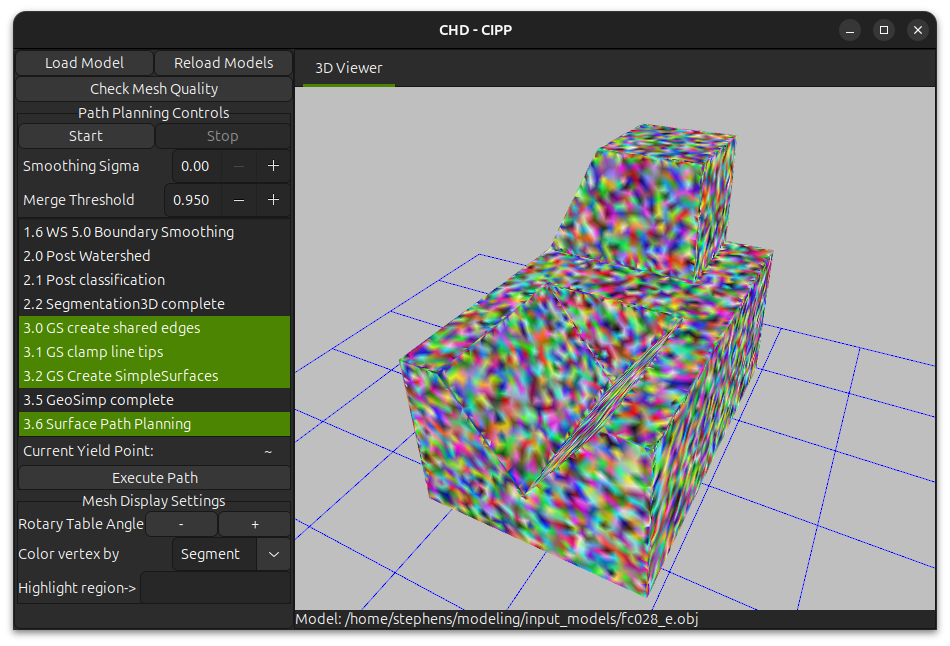
\includegraphics[width=\textwidth]{../resources/gui/gui_full_enabled.png}};
	% \node[left=of GUIFull] (GUIDisabled) {\includegraphics[width=0.2\textwidth]{../resources/gui/gui_disabled.png}};
	\node[nBalloon] at (-6,4.6) {1}; % Load model
	\node[nBalloon] at (-4,4.6) {2}; % Reload models
	\draw[draw,-{Latex[round]}] (-7.5,3.7) node[nBalloon] {3} -- +(340:3.8mm); % Check mesh quality
	% \node[nBalloon] at (-7.5,2.8) {4}; % Start
	% \node[nBalloon] at (-2.5,2.8) {5}; % Stop
	% Path planning controls
	\node[shape=rectangle,minimum height=59mm,minimum width=43mm,
		fill=gray!20,opacity=0.0] (PPControls) at (-5,0.35) {};
	\node[nBalloon,left=10mm of PPControls] (PPCnb) {4};
	\draw[nbAreaLine] (PPCnb) |- (PPControls.north west);
	\draw[nbAreaLine] (PPCnb) |- (PPControls.south west);
	% Mesh segmentation inputs
	\node[nBalloon] at (-2.5,2.37) {5}; % Smoothing sigma
	\node[nBalloon] at (-2.5,1.87) {6}; % Merge threshold
	% YieldPoint window
	\node[shape=rectangle,minimum height=34mm,minimum width=43mm,
		fill=gray!20,opacity=0.0] (YPwindow) at (-5,-0.06) {};
	\node[nBalloon,left=2mm of YPwindow] (YPnb) {7};
	\draw[nbAreaLine] (YPnb) |- (YPwindow.north west);
	\draw[nbAreaLine] (YPnb) |- (YPwindow.south west);
	% Execute path
	\node[nBalloon] at (-2.5,-2.40) {8};
	% Mesh Display Settings
	\node[shape=rectangle,minimum height=16mm,minimum width=43mm,
		fill=gray!20,opacity=0.0] (MeshDispSettings) at (-5,-3.5) {};
	\node[nBalloon,left=2mm of MeshDispSettings] (MDSnb) {9};
	\draw[nbAreaLine] (MDSnb) |- (MeshDispSettings.north west);
	\draw[nbAreaLine] (MDSnb) |- (MeshDispSettings.south west);
	% scene and model label
	\node[nBalloon] at (6,2.5) {10};
	\draw[draw,-{Latex[round]}] (-1,-3.9) node[nBalloon, in front of path] {11} -- +(270:4.5mm);
\end{tikzpicture}
	\caption{Application GUI with callouts}
	\label{fig:gui_overview}
\end{figure}

\begin{enumerate}
	\item \textbf{Load Model}: Opens a dialog box to load a 3D mesh.
		At the time of writing, only OBJ files were accepted for openeing and processing.
	\item \textbf{Reload Models}: Reloads the scene elements as well as the 3D mesh, if any.
		Throughout development various scene elements were created, mostly to represent the rotary table and robotic arm.
		The plan was to view a simulation of the robot and rotary table executing the planned path.
		% I could expand on why this was not pursued, but the short answer is the same almost all others: lack of time
	\item \textbf{Check Mesh Quality}: The initial 3D meshes used for testing were not always complete, and this led to errors in the program.
		Although the algorithm and code were later improved to be more robust when dealing with an incomplete mesh, the quick solution was to create a function to check the mesh for holes and other imperfections, and an accompanying button to trigger the mesh check.
		Mesh issues detected are printed to the terminal window that accompanies the program.
	\item \textbf{Path Planning Controls}: This panel controls the mesh segmentation settings and execution of the path planning algorithm.
		The first two buttons marked \textbf{Start} and \textbf{Stop}, start and stop execution of the path planner, respectively.
		While the path planner is inactive, the \textbf{Stop} button is disabled, indicated by being grayed out.
		Once the path planner has been started the text of the \textbf{Start} button changes to ``Continue'', and the \textbf{Stop} button is enabled.
	\item \textbf{Smoothing Sigma}: This field is used to smooth the curvature derivative values post computation.
		The smoothing value corresponds to the sigma of a Gaussian smoothing function.
		A value of 0 disables curvature smoothing.
	\item \textbf{Merge Threshold}: This field sets the initial merge threshold exponent used during Watershed segmentation in the \textit{3D Segmentation} high-level step.
		It was originally used to examined the effect of different merge thresholds during Watershed segmentation.
		Because the merge threshold is iteratively reduced during the \textit{3D Segmentation} step, this field is largely unused now.
	\item \textbf{Yield Point Window}: To facilitate debugging and displaying intermediate results ``Yield Points'' were developed.
		Yield points are similar to breakpoints used to aid in debugging a program, but do not completely interrupt execution, only the path planning procedure.
		Yield points may be activated / deactivated in by de/selecting them in the \textbf{Yield Point Window}.
		Updated mesh colors, typically to display the results of a segmentation step, are passed to yield points to update the mesh's appearance.
		This allows the user to view the evolution of the mesh's segmentation in real time, especially if the \textit{3D Segmentation} yield points are inactive.
		Below the \textbf{Yield Point Window} is a field to display the current yield point.
		When execution reaches a yield point, the path planner pauses, until \textbf{Continue} (the Start button) is clicked.
	\item \textbf{Execute Path}: Button to send commands to the robot arm.
		This button would be used to send the planned path to the robot arm and rotary table, but only basic funcitonality was tested.
		% Again, could elaborate on what it is actually / currently used for, but that will likely come in the discussion.
	\item \textbf{Mesh Display Settings}: This panel contains settings relevant to how the mesh is displayed.
		The rotary table angle controls are a remnant from when the rotary table was expected to have only 8 positions.
		Similarly, the vertex color input was created to examine different types of curvature, to determine which was best suited as the basis for Watershed segmentation.
		The \textbf{Highlight region} field is used to highlight a region specified by its index.
		The program's output log displays plenty of information detailing the results of each path planning step, but due to its textual nature mesh regions and simple surfaces are reduced to a number.
		Thus, it is necessary to have a function that ``puts a name to a face'', or a number to a mesh region, in this case.
	\item \textbf{Display Window}: This is the scene where the loaded 3D mesh is displayed.
		The ability to rotate and zoom the scene was included in the base form of the GUI application.
	\item \textbf{Model Label}: This field displays the filepath to the loaded 3D mesh.
		This is particularly useful when comparing multiple versions of the same model but with different meshes, to ensure there is no confusion as to which mesh is currently loaded.
\end{enumerate}

Altough not relevant to the research goals of this project, the application critical to development and testing.
Development of the application and its GUI took a not insignificant portion of the alloted project time, hence the need to mention it.

\section{Testing Setup}

% \subsection{Test Model Sources}
To test the algorithm developed, a collection of test meshes was sought.
The very early days of development relied on the default cube in Blender with varied mesh density.
Once Watershed segmentation yielded plausible results from the default cube, meshes from scanned objects were demanded.
To meet this request models were scoured from Fraunhofer IGD's own collection of scanned and reconstructed cultural artefacts.
All but one of the reconstructed meshes were too complex to be useful during testing.
To ensure the algorithm's generalizability additional test models were eventually sought, this time from CAD databases.
The vast majority of these came originally from Thingiverse, an online platform for users to post their 3D printable models\cite{Thingiverse}.
The full list of test models and their sources can be found in appendix \ref{App:model_table}.

\subsection{Remeshing}
Because Watershed segmentation requires input models to have a mesh of vertices upon which the height function may be computed, and CAD models store only what is required to reconstruct their geometry, remeshing was required as a pre-processing step.
PyMeshLab's ``isotropic explicit remeshing''\cite{PyMeshLab} was chosen for this purpose.
Manually varying the mesh density by model region can reduce mesh file sizes and expedite computation time without compromising the quality of the path planned, but is still typically slower than applying a high-density mesh to the entire model and accepting slower algorithm completion times.
The primary input parameter of \textit{isotropic explicit remeshing} is the ``target length'', which sets the target length of the remeshed edges as a percentage of something.
Unfortunately PyMeshLab's documentation is unclear as to what this value is a percentage of.
% I tried to find the answer, believe me.
The vast majority of test models were remeshed with a uniform ``target length'', and the remainder were remeshed using manual selection of regions.
Models that were remeshed with non-uniform target lengths have a range of values in the \textbf{Mesh} column in appendix \ref{App:model_table}.

Prior to testing each test object was examined and assigned a ``difficulty class'' from 1-4.
The difficulty classification was created during a period when the algorithm's conic regression and cylinder detection functionality were sub-optimal and required improvement.
Hence the higher difficulty class for objects with cylindric surfaces.
The example images in the following sections were created using Blender\cite{Blender}.

\subsection{Difficulty Class 1}
These objects are comprised solely of planar surfaces and should pose little to no trouble to the path planner.
Figure \ref{fig:class_1_models} shows 3 such examples.

\begin{figure}[htb]
\centering
\begin{subfigure}{0.3\textwidth}
	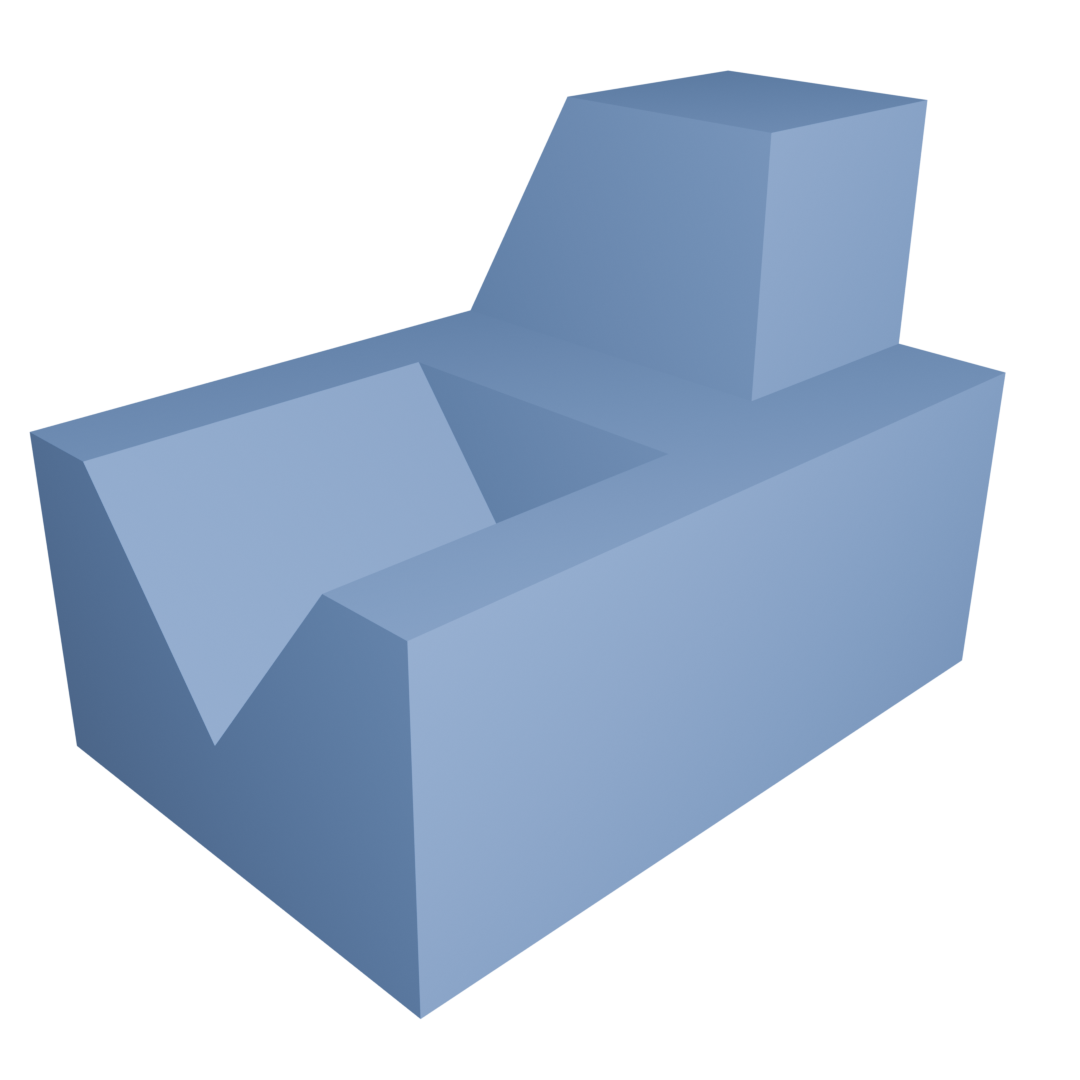
\includegraphics[width=\textwidth]{../resources/models/fc028.png}
	\caption{Model fc028}
	% \label{sfig:first}
\end{subfigure}
\hfill
\begin{subfigure}{0.3\textwidth}
	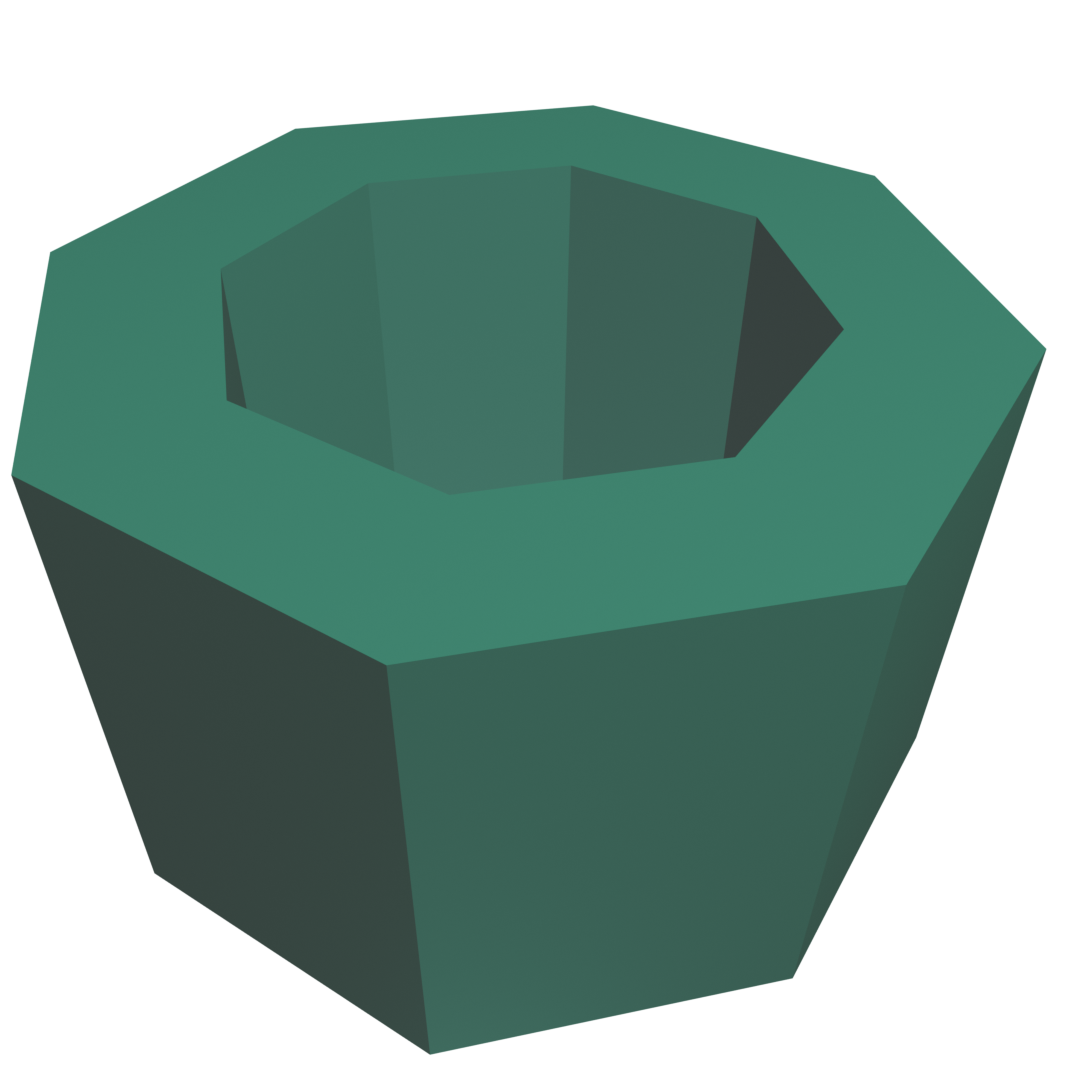
\includegraphics[width=\textwidth]{../resources/models/1505020.png}
	\caption{Model 1505020}
	% \label{sfig:second}
\end{subfigure}
\hfill
\begin{subfigure}{0.3\textwidth}
	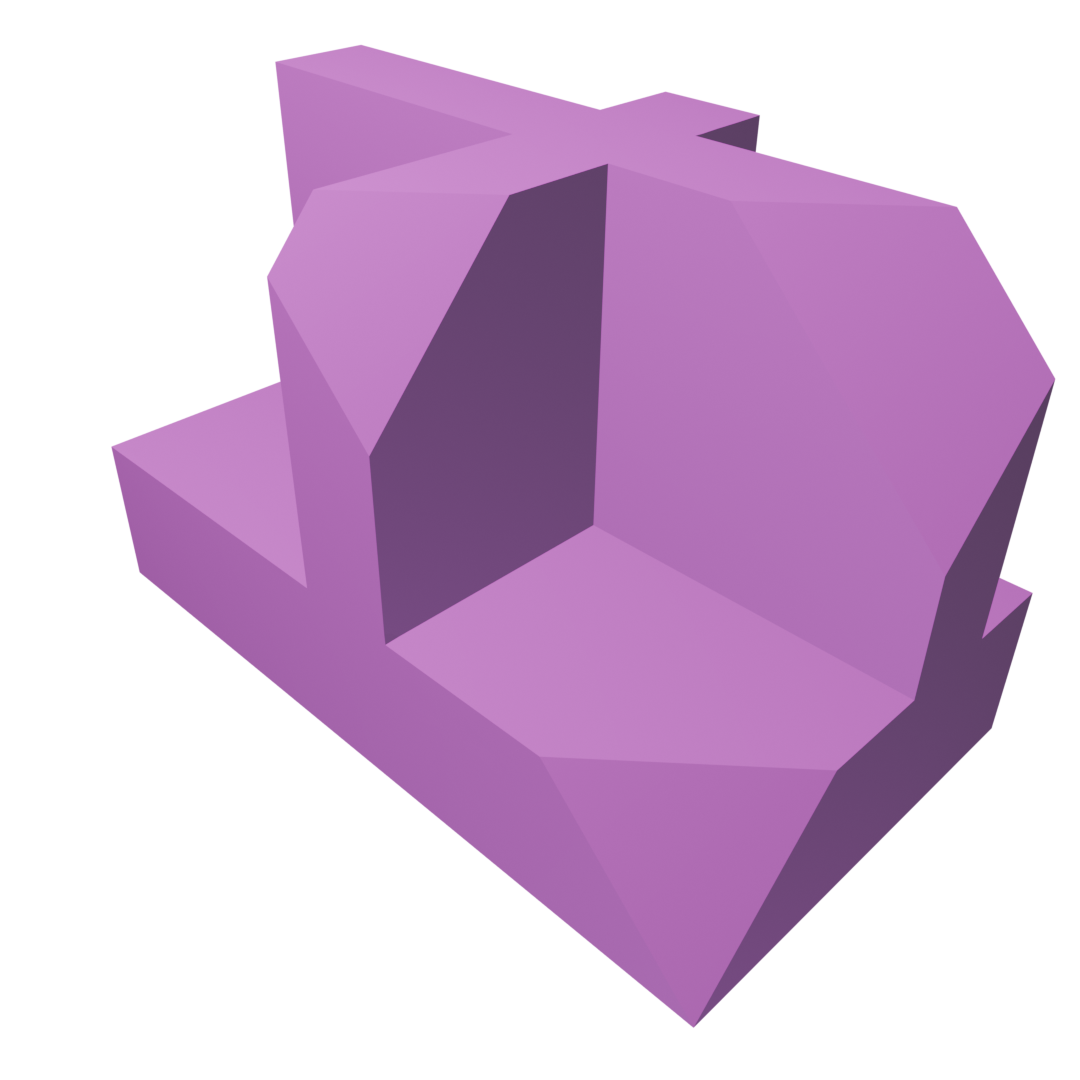
\includegraphics[width=\textwidth]{../resources/models/fc004.png}
	\caption{Model fc004}
	% \label{sfig:third}
\end{subfigure}
\caption{Test models of difficulty class 1}
\label{fig:class_1_models}
\end{figure}

\subsection{Difficulty Class 2}
Features that would cause an object to be pushed into class 2 include small or narrow surfaces, as well as cylindric surfaces.
There is a decent chance that small and thin surfaces will be absorbed into a neighboring large planar region, decreasing the chance that the combined region will be classified as planar.
Three examples of class 2 test models can be found in figure \ref{fig:class_2_models}.

\begin{figure}[htb]
\centering
\begin{subfigure}{0.3\textwidth}
	
\includegraphics[width=\textwidth]{../resources/models/55583.png}
	\caption{Model 55583}
	\label{sfig:55583}
\end{subfigure}
\hfill
\begin{subfigure}{0.3\textwidth}
	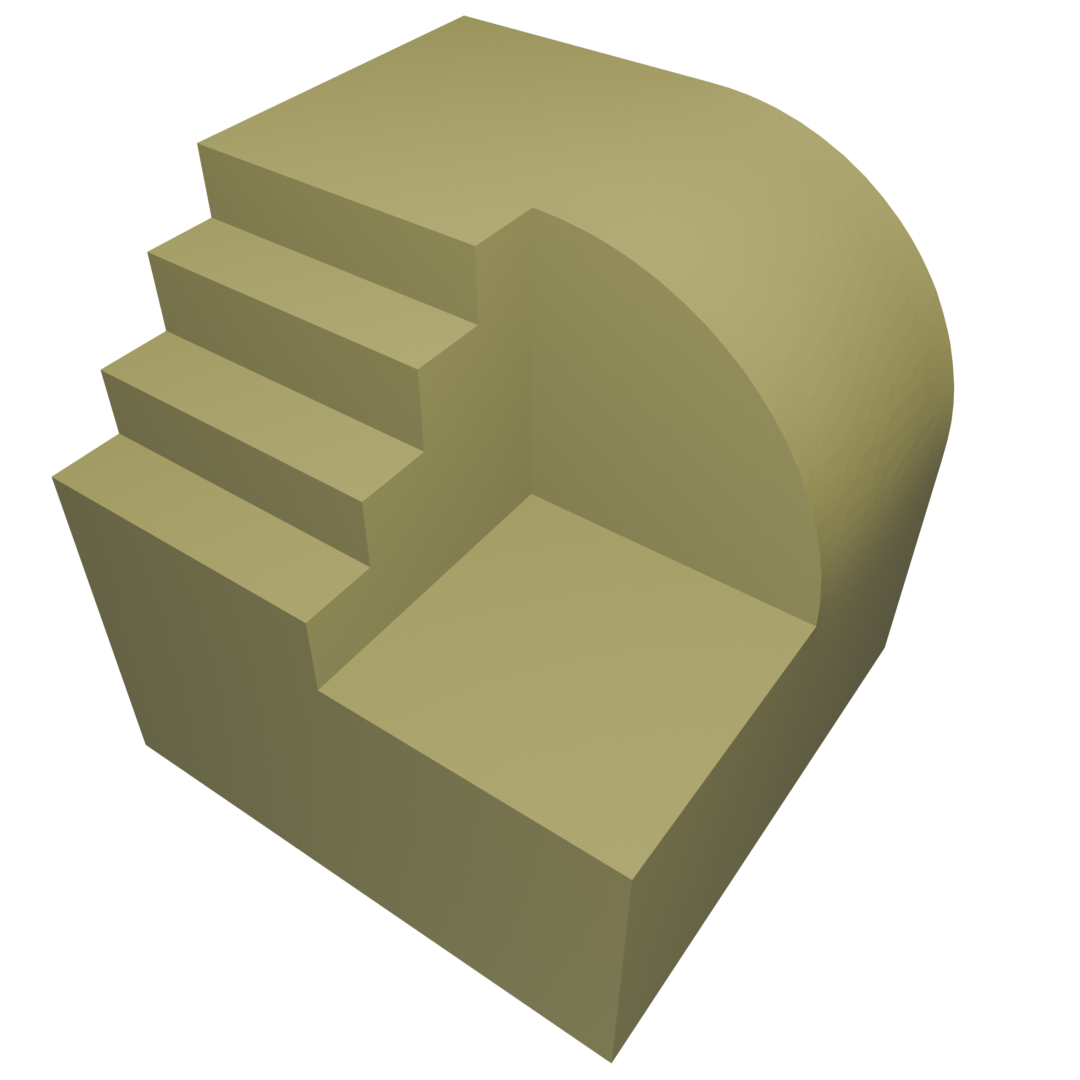
\includegraphics[width=\textwidth]{../resources/models/7120369.png}
	\caption{Model 7120369}
	\label{sfig:7120369}
\end{subfigure}
\hfill
\begin{subfigure}{0.3\textwidth}
	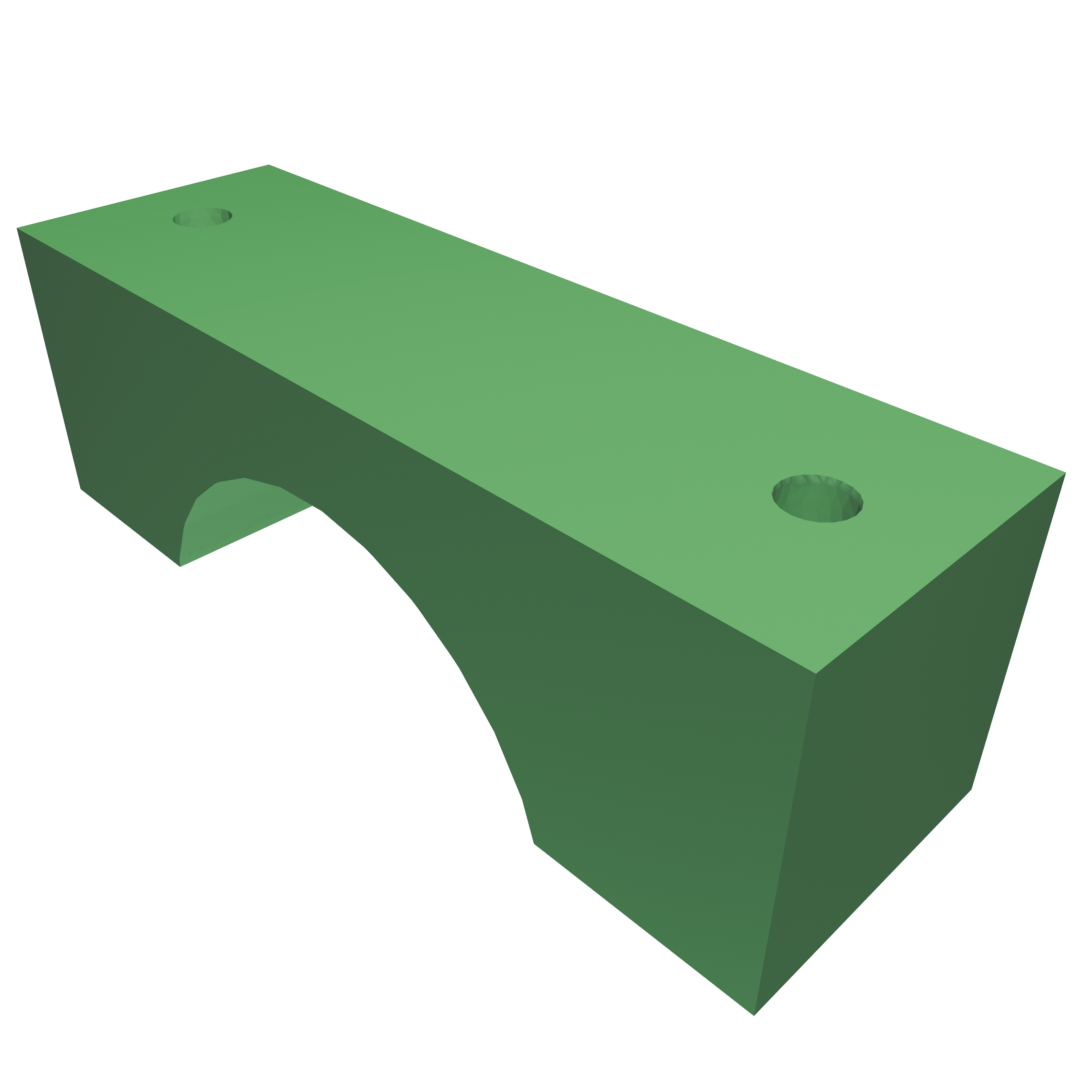
\includegraphics[width=\textwidth]{../resources/models/68501.png}
	\caption{Model 68501}
	% \label{sfig:third}
\end{subfigure}
\caption{Test models of difficulty class 2}
\label{fig:class_2_models}
\end{figure}

Of the models shown in figure \ref{fig:class_2_models} model 55583 (subfigure \ref{sfig:55583}) has the highest potential for failure, due to the narrow surfaces at the top of each gear tooth.
The smooth transitions from planar to cylindric in subfigure \ref{sfig:7120369} will also be difficult for the path planner.

\subsection{Difficulty Class 3}
Objects of this class are expected to be difficult despite improvements to cylinder detection and regression, and handling of narrow planar surfaces.
The examples shown in figure \ref{fig:class_3_models} showcase various difficult features.

\begin{figure}[htb]
\centering
\begin{subfigure}{0.3\textwidth}
	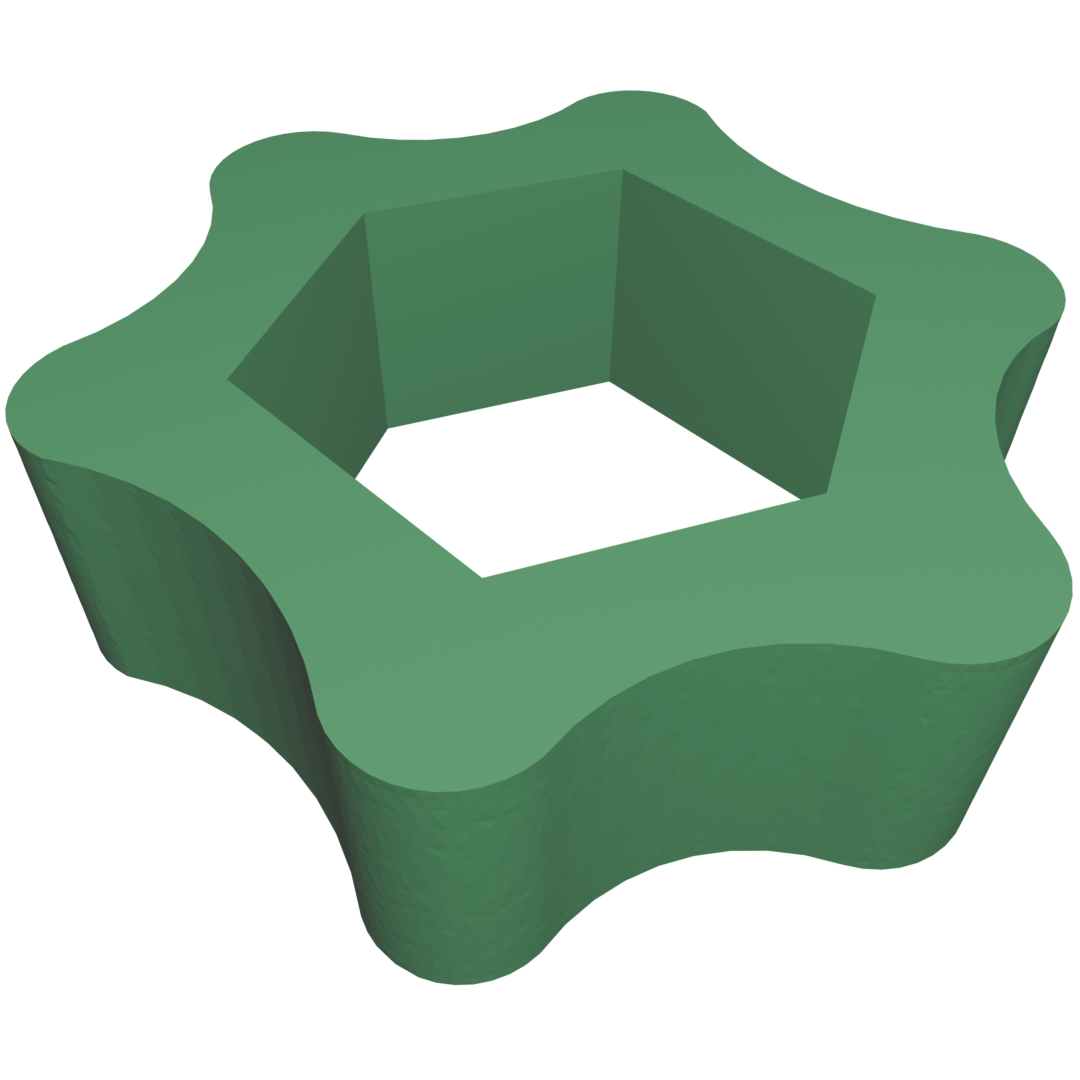
\includegraphics[width=\textwidth]{../resources/models/97733.png}
	\caption{Model 97733}
	% \label{sfig:first}
\end{subfigure}
\hfill
\begin{subfigure}{0.3\textwidth}
	
\includegraphics[width=\textwidth]{../resources/models/42042.png}
	\caption{Model 42042}
	% \label{sfig:second}
\end{subfigure}
\hfill
\begin{subfigure}{0.3\textwidth}
	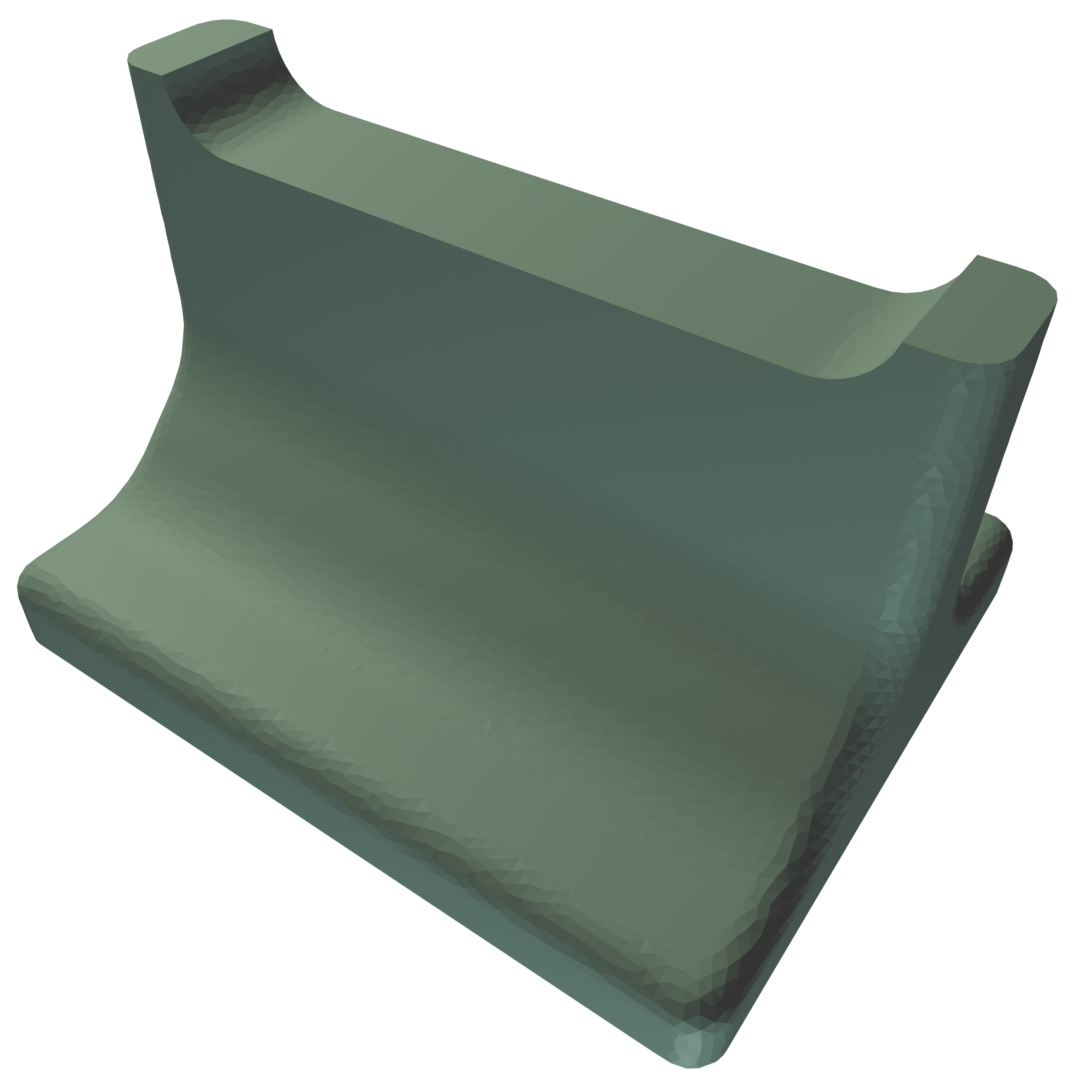
\includegraphics[width=\textwidth]{../resources/models/1148449.png}
	\caption{Model 1148449}
	% \label{sfig:third}
\end{subfigure}
\caption{Test models of difficulty class 3}
\label{fig:class_3_models}
\end{figure}

\subsection{Difficulty Class 4}
Difficulty class 4 models are beyond the scope of this work, but are included for comparison purposes.
Figure \ref{fig:class_4_models} shows a few such models.

\begin{figure}[htb]
\centering
\begin{subfigure}{0.3\textwidth}
	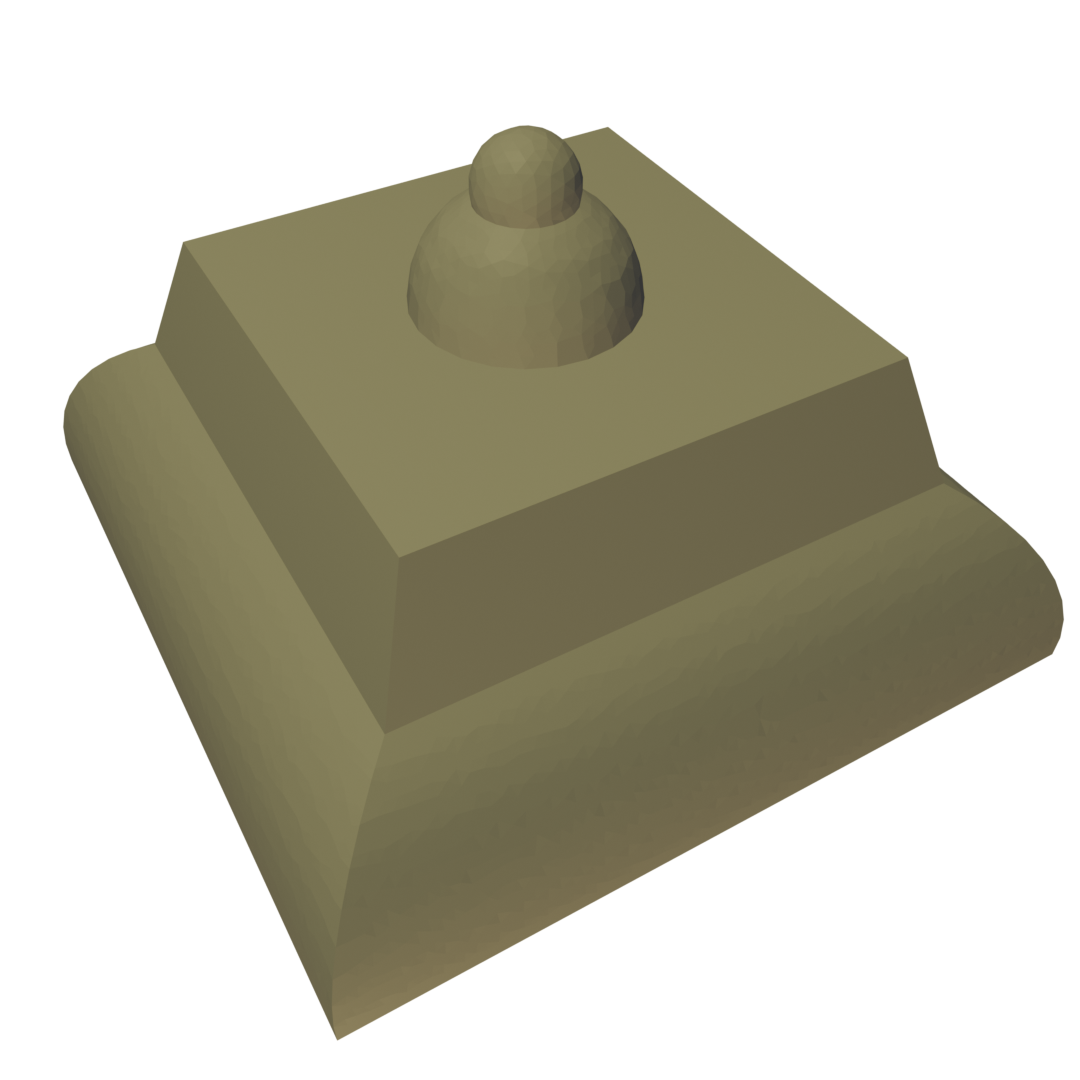
\includegraphics[width=\textwidth]{../resources/models/50704.png}
	\caption{Model 50704}
	\label{sfig:50704}
\end{subfigure}
\hfill
\begin{subfigure}{0.3\textwidth}
	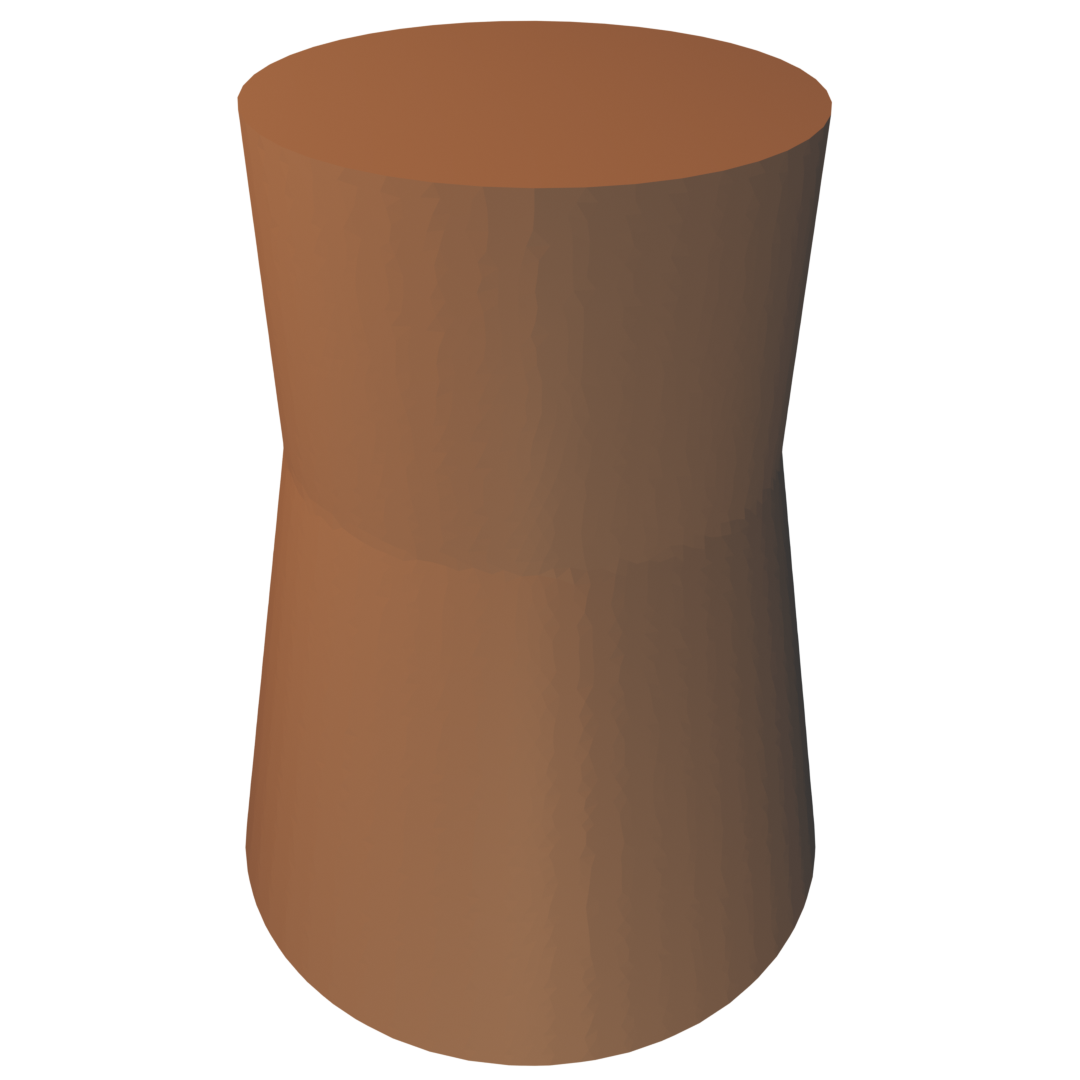
\includegraphics[width=\textwidth]{../resources/models/229605.png}
	\caption{Model 229605}
	\label{sfig:229605}
\end{subfigure}
\hfill
\begin{subfigure}{0.3\textwidth}
	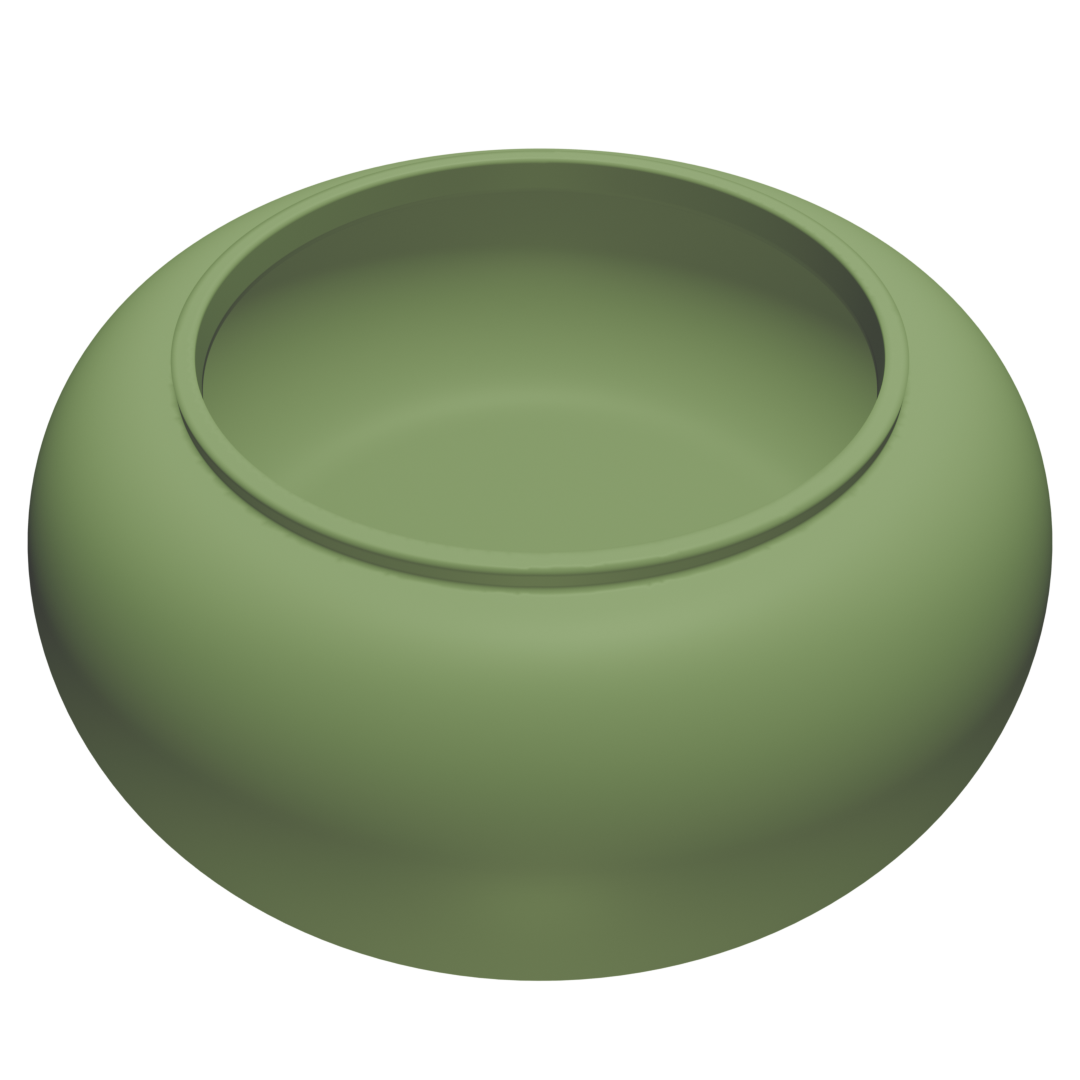
\includegraphics[width=\textwidth]{../resources/models/99265.png}
	\caption{Model 99265}
	\label{sfig:99265}
\end{subfigure}
\caption{Test models of difficulty class 4}
\label{fig:class_4_models}
\end{figure}

Although spherical surfaces, such as those adorning model 50704 (figure \ref{sfig:50704}), were part of the planned set of detectable primitives, that functionality was not completed.
Thus, even if the path planner were able to perfectly handle the curved surfaces at the base of model 50704, the partial spheres would result in a failure.
Model 229605 (subfigure \ref{sfig:229605} appears simple at first glance, but its lower half is that of a cone, and the detection thereof is not implemented.
Model 99265, shown in subfigure \ref{sfig:99265}, exhibits swept curves which the path planner is unable to process.
Its overall form, comprised of occluded regions, is also beyond the scope of the intended application of the path planner developed.

